\documentclass[11pt]{article}
\usepackage[margin=2cm]{geometry}
\usepackage{booktabs,graphicx,amsmath,amssymb,amsthm,placeins,adjustbox,threeparttable,multirow,array}
\usepackage[round,authoryear]{natbib}
\usepackage[capitalise,noabbrev]{cleveref}
\graphicspath{{figures/}}
\renewcommand\thesection{S\arabic{section}}
\counterwithin{table}{section}
\counterwithin{figure}{section}
\counterwithin{equation}{section}
\renewcommand\thetable{\thesection.\arabic{table}}
\renewcommand\thefigure{\thesection.\arabic{figure}}
\renewcommand\theequation{\thesection.\arabic{equation}}
\newcommand{\rw}{Y}
\newcommand{\uhat}{\hat{u}}
\newcommand{\Stat}{S_\theta}
\newcommand{\StatZero}{S}
\newcommand{\hacsig}{\hat{\sigma}_{\mathrm{HAC}}}
\newcommand{\ncal}{N_{\mathrm{cal}}}
\newcommand{\Nsim}{N_{\mathrm{sim}}}
\newcommand{\Fnull}{F_0}
\newcommand{\Fnullhat}{\hat{F}_0}
\newcommand{\cbar}{\bar{c}}
\newcommand{\abar}{\bar{a}}
\newcommand{\sAR}{s^2_{\mathrm{AR}}}
\newcommand{\Var}{\operatorname{Var}}
\newcommand{\E}{\mathbb{E}}
\newcommand{\Prob}{\mathbb{P}}
\newcommand{\R}{\mathbb{R}}
\newcommand{\convd}{\xrightarrow{d}}
\newcommand{\convp}{\xrightarrow{p}}
\newcommand{\weak}{\Rightarrow}
\newcommand{\iid}{\stackrel{\mathrm{iid}}{\sim}}
\newcommand{\RMGLS}{MSB-B}
\newcommand{\bm}{W}
\newcommand{\rmean}{\bar{e}}
\newcommand{\Cov}{\operatorname{Cov}}
\newcommand{\indic}[1]{\mathbf{1}\{#1\}}
\newcommand{\dgls}{DF-GLS}
\newcommand{\pending}[1]{\textcolor{red}{[#1]}}
\title{Supplementary material}
\date{}
\begin{document}
\maketitle
Sections, tables and figures are numbered S$k$ and S$k.j$. Every table is generated from the machine-readable files in \texttt{data/}; \texttt{README.md} maps each table to its source. References to the main text give the number of the table, section or equation there.

\FloatBarrier
\section{Power under i.i.d.\ errors at equalized size}\label{supp:s1}

RM: the centred rolling-means statistic with $\theta = 0.1$.

\subsection*{Size}

\Cref{tab:size} reports the size of \RMGLS{} under equation~(2) of the main text. Every
cell lies within $0.25$ points of the nominal level. The largest deviation,
$0.24$ points in the trend case at $n = 100$, is a rate of $0.0524$ that
lies just above the exact region for $5\times 10^4$ paths; the smoothed
statistic with $\theta = 0.02$ gives $0.0526$ on the same paths and an
independent replication gives $0.0493$, so the deviation belongs to the
paths and not to the statistic.

\begin{table}[t]
\centering
\caption{Size of \RMGLS{} under the Gaussian random walk, $\alpha = 0.05$,
with 95\% Wilson intervals.}
\label{tab:size}
\begin{threeparttable}
% Generado por experiments/audit13_tables.py desde e_size_audit13.json, b101_theta_audit10.json, b103_lown_audit10.json (no editar a mano)
\begin{tabular}{rcc}
\toprule
$n$ & Constant & Trend \\
\midrule
60 & 0.0507 [0.0488, 0.0526] & 0.0503 [0.0484, 0.0523] \\
100 & 0.0501 [0.0482, 0.0520] & 0.0524 [0.0504, 0.0543] \\
150 & 0.0487 [0.0469, 0.0507] & 0.0494 [0.0475, 0.0513] \\
200 & 0.0502 [0.0489, 0.0516] & 0.0499 [0.0486, 0.0513] \\
500 & 0.0492 [0.0478, 0.0505] & 0.0502 [0.0489, 0.0516] \\
1000 & 0.0491 [0.0478, 0.0505] & 0.0505 [0.0492, 0.0519] \\
\bottomrule
\end{tabular}

\begin{tablenotes}\footnotesize
\item $5\times10^4$ independent paths per cell for $n \leq 150$ and
$10^5$ for $n \geq 200$; the two deterministic cases use independent
paths; $\ncal = 5\times 10^5$.
\end{tablenotes}
\end{threeparttable}
\end{table}

\subsection*{Power in finite samples at equalized size}

\Cref{tab:dgp1,tab:ctpower} and \cref{fig:powereq} report power against
the stationary autoregression $\rw_t = \rho\rw_{t-1} + \varepsilon_t$ with
i.i.d.\ Gaussian innovations, $\rho \in \{0.80, 0.85, 0.90, 0.93, 0.95,
0.97, 0.99\}$, and, in the trend case, against the same process around a
linear trend, with every procedure at its simulated critical value.

At $n = 200$ in the constant case \RMGLS{} exceeds DF-GLS by $6.8$ points
at $\rho = 0.90$ ($0.993$ against $0.926$) and $5.6$ points at $\rho =
0.93$, both with McNemar $p < 10^{-4}$, by $3.5$ and $4.7$ points at
$\rho = 0.80$ and $0.85$, and by $1.8$ points at $\rho = 0.95$ ($p =
0.002$); it concedes $1.1$ points at $\rho = 0.97$ ($p = 0.045$). With
$n = 500$ and $1000$ the pattern moves toward the unit root, as local
asymptotics predict: \RMGLS{} is ahead at $\rho = 0.97$, $n = 500$ by $1.6$
points and behind at $\rho = 0.99$ by $1.5$ points at $n = 500$ and $1.8$
at $n = 1000$. Against ADF and PP the margin is large everywhere, up to
$43$ and $42$ points at $(\rho, n) = (0.99, 1000)$. In the trend case
\RMGLS{} leads DF-GLS by $9.9$ points at $(\rho, n) = (0.90, 200)$ and by
$6.2$ points at $(0.95, 500)$, and the two are statistically level in
five of the nine informative cells of \cref{tab:ctpower}. These are
comparisons under i.i.d.\ innovations, the only case in which every
procedure has exact size; Section~4.5 of the main text shows why they do not carry
over to serially correlated errors.

\begin{table}[t]
\centering
\caption{Power against $\rw_t = \rho\rw_{t-1} + \varepsilon_t$, constant
case, at equalized size, $\alpha = 0.05$.}
\label{tab:dgp1}
\begin{threeparttable}
\small
% Generado por experiments/audit15_supplement.py desde e_equalized_audit13.json (no editar a mano)
\begin{tabular}{rrcccccccc}
\toprule
$\rho$ & $n$ & \RMGLS{} & RM & ADF & PP & DF-GLS & MZ$_t$ & MSB & $p$ \\
\midrule
0.80 & 200 & 1.000 & 1.000 & 0.984 & 1.000 & 0.965 & 0.952 & 0.947 & $<$0.001 \\
0.85 & 200 & 1.000 & 0.994 & 0.958 & 0.995 & 0.953 & 0.944 & 0.941 & $<$0.001 \\
0.90 & 200 & 0.993 & 0.896 & 0.798 & 0.850 & 0.926 & 0.928 & 0.922 & $<$0.001 \\
0.93 & 200 & 0.910 & 0.647 & 0.491 & 0.538 & 0.854 & 0.856 & 0.835 & $<$0.001 \\
0.95 & 200 & 0.708 & 0.426 & 0.291 & 0.313 & 0.690 & 0.691 & 0.654 & 0.002 \\
0.97 & 200 & 0.386 & 0.233 & 0.147 & 0.150 & 0.397 & 0.393 & 0.365 & 0.045 \\
0.99 & 200 & 0.115 & 0.092 & 0.067 & 0.066 & 0.111 & 0.112 & 0.113 & 0.244 \\
\addlinespace
0.80 & 500 & 1.000 & 1.000 & 1.000 & 1.000 & 1.000 & 1.000 & 1.000 & 1.000 \\
0.85 & 500 & 1.000 & 1.000 & 0.999 & 1.000 & 1.000 & 1.000 & 1.000 & 1.000 \\
0.90 & 500 & 1.000 & 1.000 & 1.000 & 1.000 & 0.999 & 0.999 & 1.000 & 0.250 \\
0.93 & 500 & 1.000 & 0.999 & 0.994 & 1.000 & 0.997 & 0.996 & 0.997 & $<$0.001 \\
0.95 & 500 & 1.000 & 0.980 & 0.939 & 0.955 & 0.992 & 0.993 & 0.992 & $<$0.001 \\
0.97 & 500 & 0.955 & 0.726 & 0.577 & 0.604 & 0.939 & 0.940 & 0.934 & $<$0.001 \\
0.99 & 500 & 0.301 & 0.187 & 0.119 & 0.127 & 0.316 & 0.313 & 0.295 & 0.001 \\
\addlinespace
0.80 & 1000 & 1.000 & 1.000 & 1.000 & 1.000 & 1.000 & 1.000 & 1.000 & 1.000 \\
0.85 & 1000 & 1.000 & 1.000 & 1.000 & 1.000 & 1.000 & 1.000 & 1.000 & 1.000 \\
0.90 & 1000 & 1.000 & 1.000 & 1.000 & 1.000 & 1.000 & 1.000 & 1.000 & 1.000 \\
0.93 & 1000 & 1.000 & 1.000 & 1.000 & 1.000 & 1.000 & 1.000 & 1.000 & 1.000 \\
0.95 & 1000 & 1.000 & 1.000 & 1.000 & 1.000 & 1.000 & 1.000 & 1.000 & 1.000 \\
0.97 & 1000 & 1.000 & 0.998 & 0.992 & 0.992 & 1.000 & 1.000 & 1.000 & 1.000 \\
0.99 & 1000 & 0.737 & 0.434 & 0.303 & 0.318 & 0.755 & 0.755 & 0.728 & $<$0.001 \\
\bottomrule
\end{tabular}

\begin{tablenotes}\footnotesize
\item All comparators at simulated critical values; MZ$_t$ and MSB are
the GLS versions. $p$: exact McNemar test of \RMGLS{} against DF-GLS.
\end{tablenotes}
\end{threeparttable}
\end{table}

\begin{table}[t]
\centering
\caption{Power against a stationary autoregression around a linear
trend, trend case, at equalized size, $\alpha = 0.05$.}
\label{tab:ctpower}
\begin{threeparttable}
\small
% Generado por experiments/audit15_supplement.py desde e_equalized_audit13.json (no editar a mano)
\begin{tabular}{rrcccccccc}
\toprule
$\rho$ & $n$ & \RMGLS{} & RM & ADF & PP & DF-GLS & MZ$_t$ & MSB & $p$ \\
\midrule
0.90 & 200 & 0.819 & 0.740 & 0.556 & 0.630 & 0.720 & 0.742 & 0.734 & $<$0.001 \\
0.95 & 200 & 0.297 & 0.257 & 0.175 & 0.189 & 0.290 & 0.290 & 0.284 & 0.124 \\
0.97 & 200 & 0.132 & 0.122 & 0.098 & 0.096 & 0.130 & 0.132 & 0.130 & 0.555 \\
0.99 & 200 & 0.062 & 0.060 & 0.058 & 0.060 & 0.062 & 0.064 & 0.062 & 1.000 \\
\addlinespace
0.90 & 500 & 1.000 & 1.000 & 0.996 & 1.000 & 0.984 & 0.989 & 0.988 & $<$0.001 \\
0.95 & 500 & 0.960 & 0.913 & 0.782 & 0.815 & 0.899 & 0.911 & 0.910 & $<$0.001 \\
0.97 & 500 & 0.589 & 0.515 & 0.355 & 0.380 & 0.575 & 0.578 & 0.563 & 0.004 \\
0.99 & 500 & 0.099 & 0.089 & 0.072 & 0.075 & 0.102 & 0.103 & 0.100 & 0.311 \\
\addlinespace
0.90 & 1000 & 1.000 & 1.000 & 1.000 & 1.000 & 1.000 & 1.000 & 1.000 & 1.000 \\
0.95 & 1000 & 1.000 & 1.000 & 0.999 & 1.000 & 0.998 & 0.999 & 0.999 & 0.004 \\
0.97 & 1000 & 0.994 & 0.977 & 0.913 & 0.923 & 0.975 & 0.980 & 0.980 & $<$0.001 \\
0.99 & 1000 & 0.305 & 0.270 & 0.195 & 0.198 & 0.304 & 0.305 & 0.303 & 0.657 \\
\bottomrule
\end{tabular}

\begin{tablenotes}\footnotesize
\item As in \cref{tab:dgp1}.
\end{tablenotes}
\end{threeparttable}
\end{table}

\begin{figure}[t]
\centering
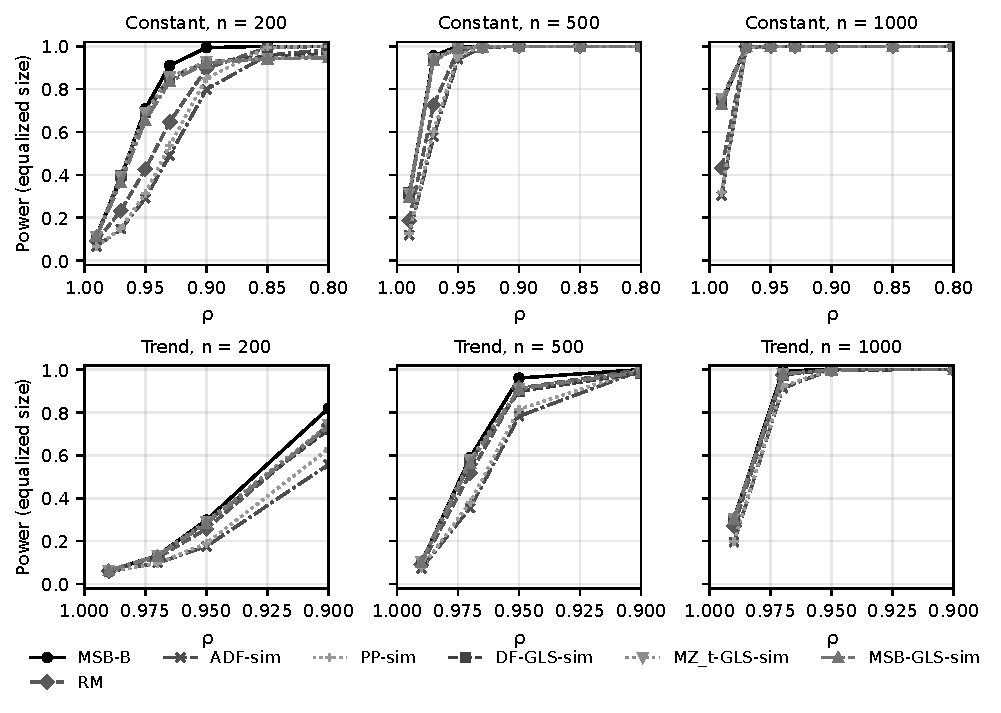
\includegraphics[width=\textwidth]{fig_power_equalized_audit13q}
\caption{Power at equalized size against $\rho$. Top row: constant case;
bottom row: trend case.}
\label{fig:powereq}
\end{figure}

\begin{figure}[t]
\centering
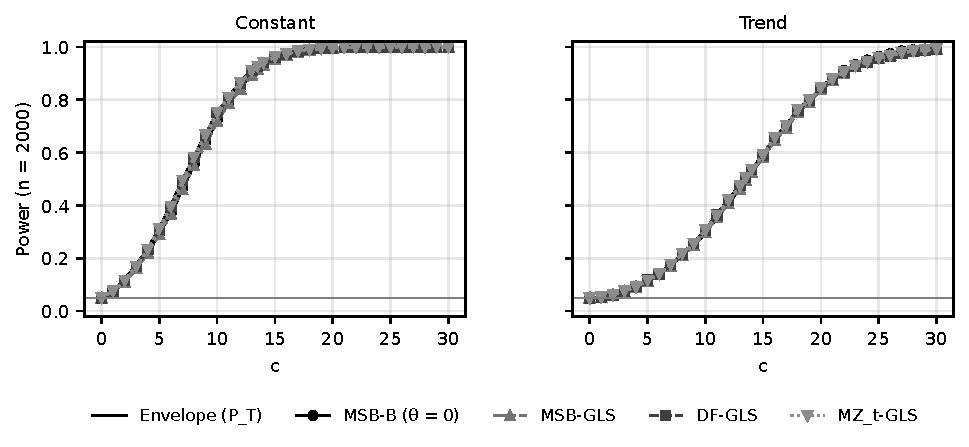
\includegraphics[width=\textwidth]{fig_local_power_audit13q}
\caption{Local asymptotic power against $c$, $n = 2000$. The curves are
within a few points of each other; Table~2 of the main text gives the
values.}
\label{fig:localpower}
\end{figure}

\FloatBarrier
\section{Serially correlated errors, cell by cell}\label{supp:s2}

The simulated critical values of MSB-GLS and MZ$_t$-GLS are exact only under equation~(2) of the main text. On the paths of \cref{tab:serial}, replacing them by the published asymptotic critical values of \citet{ng2001lag} lowers the rejection rate of both tests in all $36$ cells, by at most $0.6$ points in the constant case and by $0.4$ to $4.2$ points in the trend case. Over the $30$ cells with serial correlation the mean absolute deviation of MZ$_t$-GLS from the nominal level is $0.0142$ with simulated and $0.0130$ with asymptotic critical values. In the trend case with positive dependence and $n \leq 200$, MZ$_t$-GLS rejects between $0.062$ and $0.092$ with simulated critical values, against $0.036$ to $0.050$ with the asymptotic ones and with DF-GLS; under moving-average errors of $-0.8$ the ordering reverses, DF-GLS rejecting up to $0.142$. No test in the table controls size across the six error processes.

\begin{table}[p]
\centering
\caption{Size under a unit root with serially correlated increments,
every procedure at its critical value simulated under the i.i.d.\ null,
$\alpha = 0.05$.}
\label{tab:serial}
\footnotesize
\resizebox{\textwidth}{!}{%
% Generado por experiments/audit13_t_tables.py desde experiments/results/bA_ma_audit12.json (no editar a mano)
\begin{tabular}{lrlccccccccc}
\toprule
Errors & $n$ & Case & \RMGLS{} & (b) & (b$'$) & MSB-GLS & MZ$_t$-GLS & DF-GLS & ADF & PP & Bartlett (B) \\
\midrule
MA, $\psi = -0.8$ & 100 & Constant & \textbf{0.336} & \textbf{0.042} & \textbf{0.073} & \textbf{0.041} & \textbf{0.046} & \textbf{0.099} & \textbf{0.426} & \textbf{0.997} & 6.00 (7) \\
MA, $\psi = -0.8$ & 100 & Trend & \textbf{0.047} & \textbf{0.098} & \textbf{0.168} & \textbf{0.097} & \textbf{0.101} & \textbf{0.142} & \textbf{0.679} & \textbf{1.000} & 6.00 (7) \\
MA, $\psi = -0.8$ & 200 & Constant & \textbf{0.420} & \textbf{0.026} & \textbf{0.031} & \textbf{0.025} & \textbf{0.030} & \textbf{0.090} & \textbf{0.247} & \textbf{0.994} & 5.44 (8) \\
MA, $\psi = -0.8$ & 200 & Trend & \textbf{0.361} & \textbf{0.032} & 0.047 & \textbf{0.032} & \textbf{0.035} & \textbf{0.089} & \textbf{0.415} & \textbf{1.000} & 5.44 (8) \\
MA, $\psi = -0.8$ & 500 & Constant & \textbf{0.397} & \textbf{0.033} & \textbf{0.032} & \textbf{0.033} & \textbf{0.038} & \textbf{0.085} & \textbf{0.132} & \textbf{0.985} & 4.33 (11) \\
MA, $\psi = -0.8$ & 500 & Trend & \textbf{0.570} & \textbf{0.013} & \textbf{0.016} & \textbf{0.013} & \textbf{0.015} & \textbf{0.080} & \textbf{0.210} & \textbf{1.000} & 4.33 (11) \\
\addlinespace
MA, $\psi = -0.5$ & 100 & Constant & \textbf{0.079} & \textbf{0.054} & \textbf{0.059} & \textbf{0.053} & \textbf{0.058} & \textbf{0.067} & \textbf{0.112} & \textbf{0.575} & 1.57 (6) \\
MA, $\psi = -0.5$ & 100 & Trend & \textbf{0.026} & \textbf{0.070} & \textbf{0.083} & \textbf{0.069} & \textbf{0.072} & \textbf{0.074} & \textbf{0.184} & \textbf{0.854} & 1.57 (6) \\
MA, $\psi = -0.5$ & 200 & Constant & \textbf{0.096} & \textbf{0.058} & \textbf{0.057} & \textbf{0.057} & \textbf{0.061} & \textbf{0.065} & \textbf{0.085} & \textbf{0.517} & 1.50 (7) \\
MA, $\psi = -0.5$ & 200 & Trend & \textbf{0.071} & \textbf{0.058} & \textbf{0.063} & \textbf{0.057} & \textbf{0.059} & \textbf{0.064} & \textbf{0.116} & \textbf{0.816} & 1.50 (7) \\
MA, $\psi = -0.5$ & 500 & Constant & \textbf{0.090} & \textbf{0.056} & \textbf{0.055} & \textbf{0.055} & \textbf{0.058} & \textbf{0.060} & \textbf{0.066} & \textbf{0.402} & 1.40 (9) \\
MA, $\psi = -0.5$ & 500 & Trend & \textbf{0.097} & \textbf{0.057} & \textbf{0.057} & \textbf{0.057} & \textbf{0.056} & \textbf{0.059} & \textbf{0.078} & \textbf{0.709} & 1.40 (9) \\
\addlinespace
MA, $\psi = 0$ & 100 & Constant & 0.052 & 0.052 & 0.052 & 0.051 & \textbf{0.053} & 0.053 & 0.052 & 0.051 & 1.00 (2) \\
MA, $\psi = 0$ & 100 & Trend & 0.049 & 0.048 & 0.048 & 0.047 & 0.048 & 0.047 & 0.050 & 0.050 & 1.00 (2) \\
MA, $\psi = 0$ & 200 & Constant & 0.050 & 0.050 & 0.050 & 0.050 & 0.050 & 0.050 & 0.048 & 0.049 & 1.00 (2) \\
MA, $\psi = 0$ & 200 & Trend & 0.048 & \textbf{0.046} & \textbf{0.046} & \textbf{0.046} & \textbf{0.046} & \textbf{0.046} & 0.050 & 0.049 & 1.00 (2) \\
MA, $\psi = 0$ & 500 & Constant & 0.050 & 0.050 & 0.049 & 0.050 & 0.049 & 0.049 & 0.051 & 0.051 & 1.00 (2) \\
MA, $\psi = 0$ & 500 & Trend & 0.052 & 0.052 & 0.052 & 0.052 & 0.053 & 0.052 & 0.051 & 0.051 & 1.00 (2) \\
\addlinespace
MA, $\psi = 0.5$ & 100 & Constant & \textbf{0.027} & \textbf{0.063} & \textbf{0.061} & \textbf{0.063} & \textbf{0.063} & \textbf{0.043} & \textbf{0.056} & \textbf{0.024} & 0.93 (5) \\
MA, $\psi = 0.5$ & 100 & Trend & \textbf{0.011} & \textbf{0.086} & \textbf{0.078} & \textbf{0.086} & \textbf{0.084} & \textbf{0.036} & \textbf{0.063} & \textbf{0.009} & 0.93 (5) \\
MA, $\psi = 0.5$ & 200 & Constant & \textbf{0.032} & 0.053 & 0.051 & \textbf{0.053} & 0.052 & \textbf{0.043} & 0.050 & \textbf{0.024} & 0.94 (7) \\
MA, $\psi = 0.5$ & 200 & Trend & \textbf{0.019} & \textbf{0.063} & \textbf{0.060} & \textbf{0.064} & \textbf{0.062} & \textbf{0.036} & 0.052 & \textbf{0.009} & 0.94 (7) \\
MA, $\psi = 0.5$ & 500 & Constant & \textbf{0.040} & \textbf{0.056} & \textbf{0.055} & \textbf{0.056} & \textbf{0.053} & 0.049 & 0.050 & \textbf{0.033} & 0.96 (9) \\
MA, $\psi = 0.5$ & 500 & Trend & \textbf{0.029} & \textbf{0.058} & \textbf{0.056} & \textbf{0.058} & \textbf{0.056} & \textbf{0.045} & 0.050 & \textbf{0.018} & 0.96 (9) \\
\addlinespace
AR, $\phi = -0.5$ & 100 & Constant & \textbf{0.035} & \textbf{0.041} & \textbf{0.041} & \textbf{0.041} & \textbf{0.040} & \textbf{0.045} & 0.050 & \textbf{0.375} & 1.17 (7) \\
AR, $\phi = -0.5$ & 100 & Trend & \textbf{0.005} & \textbf{0.033} & \textbf{0.033} & \textbf{0.034} & \textbf{0.034} & \textbf{0.044} & \textbf{0.053} & \textbf{0.645} & 1.17 (7) \\
AR, $\phi = -0.5$ & 200 & Constant & \textbf{0.043} & \textbf{0.042} & \textbf{0.042} & \textbf{0.042} & \textbf{0.043} & \textbf{0.046} & 0.048 & \textbf{0.308} & 1.13 (9) \\
AR, $\phi = -0.5$ & 200 & Trend & \textbf{0.021} & \textbf{0.038} & \textbf{0.039} & \textbf{0.038} & \textbf{0.040} & \textbf{0.047} & \textbf{0.047} & \textbf{0.562} & 1.13 (9) \\
AR, $\phi = -0.5$ & 500 & Constant & \textbf{0.054} & 0.048 & 0.048 & 0.048 & 0.047 & 0.049 & 0.052 & \textbf{0.227} & 1.11 (11) \\
AR, $\phi = -0.5$ & 500 & Trend & \textbf{0.042} & \textbf{0.044} & \textbf{0.044} & \textbf{0.044} & \textbf{0.045} & 0.049 & 0.047 & \textbf{0.420} & 1.11 (11) \\
\addlinespace
AR, $\phi = 0.5$ & 100 & Constant & \textbf{0.017} & \textbf{0.070} & \textbf{0.068} & \textbf{0.071} & \textbf{0.067} & 0.048 & 0.053 & \textbf{0.022} & 0.83 (7) \\
AR, $\phi = 0.5$ & 100 & Trend & \textbf{0.004} & \textbf{0.096} & \textbf{0.092} & \textbf{0.097} & \textbf{0.092} & \textbf{0.044} & 0.049 & \textbf{0.007} & 0.83 (7) \\
AR, $\phi = 0.5$ & 200 & Constant & \textbf{0.026} & \textbf{0.059} & \textbf{0.058} & \textbf{0.058} & \textbf{0.060} & 0.052 & 0.051 & \textbf{0.022} & 0.85 (8) \\
AR, $\phi = 0.5$ & 200 & Trend & \textbf{0.010} & \textbf{0.073} & \textbf{0.073} & \textbf{0.074} & \textbf{0.073} & 0.050 & 0.050 & \textbf{0.006} & 0.85 (8) \\
AR, $\phi = 0.5$ & 500 & Constant & \textbf{0.031} & \textbf{0.055} & \textbf{0.055} & \textbf{0.054} & 0.052 & 0.049 & 0.049 & \textbf{0.027} & 0.89 (11) \\
AR, $\phi = 0.5$ & 500 & Trend & \textbf{0.021} & \textbf{0.060} & \textbf{0.061} & \textbf{0.060} & \textbf{0.060} & 0.053 & 0.051 & \textbf{0.012} & 0.89 (11) \\
\bottomrule
\end{tabular}
}
\par\medskip\begin{minipage}{\textwidth}\footnotesize
$2\times10^4$ paths per cell, common to all columns of a row; $\ncal =
5\times10^5$. (b): the numerator of \RMGLS{} scaled by $s^2_{\mathrm{AR}}$
with MAIC on GLS-detrended data; (b$'$): lag selected on OLS-detrended data
\citep{perron2007simple}. MSB-GLS, MZ$_t$-GLS and DF-GLS use the MAIC of
\citet{ng2001lag}. Last column: population factor
$\bar\sigma^2_B/\omega^2$ of Remark~2 of the main text at the median bandwidth $B$
(in parentheses). Bold: outside the exact region $[0.0470, 0.05305]$ for
$2\times10^4$ paths.
\end{minipage}
\end{table}

\begin{table}[htbp]
\centering
\caption{Size with simulated (iid) and published asymptotic critical values.}
\label{tab:serialasy}
\small
\begin{adjustbox}{max width=\textwidth}
% Generado por experiments/audit15_tables.py desde b0_iidasy_audit15.json (no editar a mano)
\begin{tabular}{lrlcccccccccc}
\toprule
& & & \multicolumn{2}{c}{MSB-GLS} & \multicolumn{2}{c}{MZ$_t$-GLS} & \multicolumn{2}{c}{MSB-GLS (PQ)} & \multicolumn{2}{c}{MZ$_t$-GLS (PQ)} & \multicolumn{2}{c}{DF-GLS}\\
\cmidrule(lr){4-5}\cmidrule(lr){6-7}\cmidrule(lr){8-9}\cmidrule(lr){10-11}\cmidrule(lr){12-13}
Errors & $n$ & Case & iid & asy. & iid & asy. & iid & asy. & iid & asy. & iid & asy.\\
\midrule
MA, $\psi = -0.8$ & 100 & Constant & \textbf{0.041} & \textbf{0.040} & \textbf{0.046} & \textbf{0.044} & \textbf{0.072} & \textbf{0.071} & \textbf{0.076} & \textbf{0.075} & \textbf{0.099} & \textbf{0.106} \\
MA, $\psi = -0.8$ & 100 & Trend & \textbf{0.097} & \textbf{0.076} & \textbf{0.101} & \textbf{0.078} & \textbf{0.167} & \textbf{0.140} & \textbf{0.170} & \textbf{0.142} & \textbf{0.142} & \textbf{0.132} \\
MA, $\psi = -0.8$ & 200 & Constant & \textbf{0.025} & \textbf{0.023} & \textbf{0.030} & \textbf{0.028} & \textbf{0.031} & \textbf{0.028} & \textbf{0.036} & \textbf{0.032} & \textbf{0.090} & \textbf{0.092} \\
MA, $\psi = -0.8$ & 200 & Trend & \textbf{0.032} & \textbf{0.023} & \textbf{0.035} & \textbf{0.024} & \textbf{0.047} & \textbf{0.035} & 0.049 & \textbf{0.036} & \textbf{0.089} & \textbf{0.073} \\
MA, $\psi = -0.8$ & 500 & Constant & \textbf{0.033} & \textbf{0.028} & \textbf{0.038} & \textbf{0.033} & \textbf{0.032} & \textbf{0.027} & \textbf{0.038} & \textbf{0.032} & \textbf{0.085} & \textbf{0.084} \\
MA, $\psi = -0.8$ & 500 & Trend & \textbf{0.013} & \textbf{0.009} & \textbf{0.015} & \textbf{0.010} & \textbf{0.016} & \textbf{0.011} & \textbf{0.018} & \textbf{0.011} & \textbf{0.080} & \textbf{0.062} \\
\addlinespace
MA, $\psi = -0.5$ & 100 & Constant & \textbf{0.053} & 0.050 & \textbf{0.058} & \textbf{0.054} & \textbf{0.058} & \textbf{0.056} & \textbf{0.062} & \textbf{0.060} & \textbf{0.067} & \textbf{0.073} \\
MA, $\psi = -0.5$ & 100 & Trend & \textbf{0.069} & \textbf{0.039} & \textbf{0.072} & \textbf{0.039} & \textbf{0.082} & 0.051 & \textbf{0.084} & 0.051 & \textbf{0.074} & \textbf{0.066} \\
MA, $\psi = -0.5$ & 200 & Constant & \textbf{0.057} & 0.052 & \textbf{0.061} & \textbf{0.056} & \textbf{0.057} & 0.052 & \textbf{0.061} & \textbf{0.057} & \textbf{0.065} & \textbf{0.066} \\
MA, $\psi = -0.5$ & 200 & Trend & \textbf{0.057} & \textbf{0.034} & \textbf{0.059} & \textbf{0.034} & \textbf{0.062} & \textbf{0.039} & \textbf{0.064} & \textbf{0.039} & \textbf{0.064} & 0.049 \\
MA, $\psi = -0.5$ & 500 & Constant & \textbf{0.055} & 0.050 & \textbf{0.058} & \textbf{0.054} & \textbf{0.055} & 0.049 & \textbf{0.059} & 0.053 & \textbf{0.060} & \textbf{0.059} \\
MA, $\psi = -0.5$ & 500 & Trend & \textbf{0.057} & \textbf{0.040} & \textbf{0.056} & \textbf{0.040} & \textbf{0.057} & \textbf{0.040} & \textbf{0.056} & \textbf{0.041} & \textbf{0.059} & 0.047 \\
\addlinespace
MA, $\psi = 0$ & 100 & Constant & 0.051 & 0.049 & \textbf{0.053} & 0.049 & 0.053 & 0.050 & 0.052 & 0.049 & 0.053 & \textbf{0.057} \\
MA, $\psi = 0$ & 100 & Trend & 0.047 & \textbf{0.020} & 0.048 & \textbf{0.019} & 0.048 & \textbf{0.023} & 0.049 & \textbf{0.021} & 0.047 & \textbf{0.041} \\
MA, $\psi = 0$ & 200 & Constant & 0.050 & \textbf{0.045} & 0.050 & \textbf{0.045} & 0.050 & \textbf{0.045} & 0.050 & \textbf{0.046} & 0.050 & 0.051 \\
MA, $\psi = 0$ & 200 & Trend & \textbf{0.046} & \textbf{0.027} & \textbf{0.046} & \textbf{0.026} & \textbf{0.046} & \textbf{0.028} & \textbf{0.047} & \textbf{0.028} & \textbf{0.046} & \textbf{0.035} \\
MA, $\psi = 0$ & 500 & Constant & 0.050 & \textbf{0.044} & 0.049 & \textbf{0.045} & 0.049 & \textbf{0.043} & 0.049 & \textbf{0.045} & 0.049 & 0.049 \\
MA, $\psi = 0$ & 500 & Trend & 0.052 & \textbf{0.036} & 0.053 & \textbf{0.036} & 0.052 & \textbf{0.036} & 0.053 & \textbf{0.035} & 0.052 & \textbf{0.041} \\
\addlinespace
MA, $\psi = 0.5$ & 100 & Constant & \textbf{0.063} & \textbf{0.060} & \textbf{0.063} & \textbf{0.058} & \textbf{0.061} & \textbf{0.058} & \textbf{0.060} & \textbf{0.057} & \textbf{0.043} & 0.047 \\
MA, $\psi = 0.5$ & 100 & Trend & \textbf{0.086} & 0.048 & \textbf{0.084} & \textbf{0.044} & \textbf{0.078} & \textbf{0.045} & \textbf{0.077} & \textbf{0.041} & \textbf{0.036} & \textbf{0.030} \\
MA, $\psi = 0.5$ & 200 & Constant & \textbf{0.053} & 0.048 & 0.052 & 0.048 & 0.051 & 0.047 & 0.051 & \textbf{0.047} & \textbf{0.043} & \textbf{0.044} \\
MA, $\psi = 0.5$ & 200 & Trend & \textbf{0.064} & \textbf{0.038} & \textbf{0.062} & \textbf{0.036} & \textbf{0.060} & \textbf{0.037} & \textbf{0.060} & \textbf{0.035} & \textbf{0.036} & \textbf{0.027} \\
MA, $\psi = 0.5$ & 500 & Constant & \textbf{0.056} & 0.050 & \textbf{0.053} & 0.049 & \textbf{0.055} & 0.050 & \textbf{0.054} & 0.049 & 0.049 & 0.048 \\
MA, $\psi = 0.5$ & 500 & Trend & \textbf{0.058} & \textbf{0.040} & \textbf{0.056} & \textbf{0.038} & \textbf{0.056} & \textbf{0.038} & \textbf{0.054} & \textbf{0.037} & \textbf{0.045} & \textbf{0.033} \\
\addlinespace
AR, $\phi = -0.5$ & 100 & Constant & \textbf{0.041} & \textbf{0.038} & \textbf{0.040} & \textbf{0.037} & \textbf{0.041} & \textbf{0.038} & \textbf{0.041} & \textbf{0.039} & \textbf{0.045} & 0.050 \\
AR, $\phi = -0.5$ & 100 & Trend & \textbf{0.034} & \textbf{0.014} & \textbf{0.034} & \textbf{0.013} & \textbf{0.033} & \textbf{0.016} & \textbf{0.034} & \textbf{0.016} & \textbf{0.044} & \textbf{0.037} \\
AR, $\phi = -0.5$ & 200 & Constant & \textbf{0.042} & \textbf{0.038} & \textbf{0.043} & \textbf{0.039} & \textbf{0.042} & \textbf{0.038} & \textbf{0.044} & \textbf{0.040} & \textbf{0.046} & \textbf{0.047} \\
AR, $\phi = -0.5$ & 200 & Trend & \textbf{0.038} & \textbf{0.020} & \textbf{0.040} & \textbf{0.019} & \textbf{0.039} & \textbf{0.022} & \textbf{0.040} & \textbf{0.022} & \textbf{0.047} & \textbf{0.035} \\
AR, $\phi = -0.5$ & 500 & Constant & 0.048 & \textbf{0.042} & 0.047 & \textbf{0.043} & 0.048 & \textbf{0.043} & 0.048 & \textbf{0.043} & 0.049 & 0.048 \\
AR, $\phi = -0.5$ & 500 & Trend & \textbf{0.044} & \textbf{0.030} & \textbf{0.045} & \textbf{0.029} & \textbf{0.044} & \textbf{0.030} & \textbf{0.045} & \textbf{0.029} & 0.049 & \textbf{0.037} \\
\addlinespace
AR, $\phi = 0.5$ & 100 & Constant & \textbf{0.071} & \textbf{0.066} & \textbf{0.067} & \textbf{0.063} & \textbf{0.068} & \textbf{0.065} & \textbf{0.065} & \textbf{0.062} & 0.048 & \textbf{0.053} \\
AR, $\phi = 0.5$ & 100 & Trend & \textbf{0.097} & \textbf{0.055} & \textbf{0.092} & 0.050 & \textbf{0.093} & \textbf{0.055} & \textbf{0.090} & 0.051 & \textbf{0.044} & \textbf{0.037} \\
AR, $\phi = 0.5$ & 200 & Constant & \textbf{0.058} & \textbf{0.054} & \textbf{0.060} & \textbf{0.055} & \textbf{0.058} & \textbf{0.054} & \textbf{0.058} & \textbf{0.054} & 0.052 & 0.053 \\
AR, $\phi = 0.5$ & 200 & Trend & \textbf{0.074} & \textbf{0.046} & \textbf{0.073} & \textbf{0.043} & \textbf{0.072} & \textbf{0.047} & \textbf{0.072} & \textbf{0.045} & 0.050 & \textbf{0.039} \\
AR, $\phi = 0.5$ & 500 & Constant & \textbf{0.054} & 0.049 & 0.052 & \textbf{0.047} & \textbf{0.054} & 0.048 & 0.052 & \textbf{0.046} & 0.049 & 0.048 \\
AR, $\phi = 0.5$ & 500 & Trend & \textbf{0.060} & \textbf{0.043} & \textbf{0.060} & \textbf{0.041} & \textbf{0.061} & \textbf{0.043} & \textbf{0.060} & \textbf{0.042} & 0.053 & \textbf{0.041} \\
\bottomrule
\end{tabular}

\end{adjustbox}
\par\medskip\begin{minipage}{\textwidth}\footnotesize Same paths as \cref{tab:serial}; asymptotic critical values of \citet{ng2001lag}.\end{minipage}
\end{table}

\begin{table}[htbp]
\centering
\caption{Size by the lag chosen by the GLS MAIC.}
\label{tab:lag}
\small
\begin{adjustbox}{max width=\textwidth}
% Generado por experiments/audit15_tables.py desde b0b_lag_audit15.json (no editar a mano)
\begin{tabular}{lrrcccc}
\toprule
& & & \multicolumn{2}{c}{MZ$_t$-GLS} & \multicolumn{2}{c}{MSB-GLS}\\
\cmidrule(lr){4-5}\cmidrule(lr){6-7}
Cell & $k$ & Paths & iid & asy. & iid & asy.\\
\midrule
AR, $\phi = 0.5$, $n = 100$, Trend & 0 & 106 & 0.028 & 0.019 & 0.028 & 0.019 \\
 & 1 & 14339 & 0.103 & 0.056 & 0.107 & 0.061 \\
 & 2 & 2391 & 0.087 & 0.045 & 0.096 & 0.053 \\
 & $\geq 3$ & 3164 & 0.051 & 0.025 & 0.052 & 0.030 \\
\addlinespace
MA, $\psi = 0.5$, $n = 100$, Trend & 0 & 180 & 0.094 & 0.039 & 0.094 & 0.039 \\
 & 1 & 3473 & 0.130 & 0.075 & 0.136 & 0.081 \\
 & 2 & 10624 & 0.085 & 0.043 & 0.084 & 0.045 \\
 & $\geq 3$ & 5723 & 0.054 & 0.029 & 0.057 & 0.032 \\
\addlinespace
MA, $\psi = -0.8$, $n = 200$, Constant & 0 & 0 & -- & -- & -- & -- \\
 & 1 & 0 & -- & -- & -- & -- \\
 & 2 & 5 & 0.200 & 0.200 & 0.200 & 0.200 \\
 & $\geq 3$ & 19995 & 0.030 & 0.028 & 0.025 & 0.023 \\
\addlinespace
MA, $\psi = 0$, $n = 100$, Trend & 0 & 14779 & 0.054 & 0.022 & 0.053 & 0.023 \\
 & 1 & 2121 & 0.043 & 0.014 & 0.039 & 0.017 \\
 & 2 & 1131 & 0.031 & 0.013 & 0.033 & 0.013 \\
 & $\geq 3$ & 1969 & 0.018 & 0.007 & 0.021 & 0.010 \\
\addlinespace
iid null (A10), $n = 100$, Trend & 0 & 367850 & 0.057 & 0.025 & 0.057 & 0.026 \\
 & 1 & 54095 & 0.039 & 0.015 & 0.038 & 0.015 \\
 & 2 & 29467 & 0.028 & 0.009 & 0.028 & 0.009 \\
 & $\geq 3$ & 48588 & 0.021 & 0.011 & 0.023 & 0.012 \\
\addlinespace
iid null (A10), $n = 200$, Constant & 0 & 357836 & 0.052 & 0.048 & 0.053 & 0.048 \\
 & 1 & 55776 & 0.048 & 0.043 & 0.047 & 0.042 \\
 & 2 & 29079 & 0.046 & 0.042 & 0.045 & 0.041 \\
 & $\geq 3$ & 57309 & 0.040 & 0.035 & 0.039 & 0.035 \\
\bottomrule
\end{tabular}

\end{adjustbox}
\end{table}

\begin{table}[htbp]
\centering
\caption{Size of MZ$_t$-GLS with five calibrations over the thirty-six designs, $\alpha = 0.05$.}
\label{tab:boot}
\small
\begin{adjustbox}{max width=\textwidth}
% Generado por experiments/audit15_v17_tables.py desde b1_boot_audit15.json (no editar a mano)
\begin{tabular}{lrlccccc}
\toprule
Errors & $n$ & Case & (i) & (ii) & (iii) & (iv) & (v$'$) \\
\midrule
MA, $\psi = -0.8$ & 100 & Constant & \textbf{0.041} & \textbf{0.043} & 0.047 & \textbf{0.037} & \textbf{0.043} \\
MA, $\psi = -0.8$ & 100 & Trend & \textbf{0.083} & \textbf{0.108} & \textbf{0.088} & \textbf{0.091} & \textbf{0.085} \\
MA, $\psi = -0.8$ & 200 & Constant & \textbf{0.028} & \textbf{0.030} & 0.048 & \textbf{0.025} & 0.046 \\
MA, $\psi = -0.8$ & 200 & Trend & \textbf{0.023} & \textbf{0.034} & \textbf{0.035} & \textbf{0.028} & \textbf{0.035} \\
MA, $\psi = -0.8$ & 500 & Constant & \textbf{0.036} & \textbf{0.040} & \textbf{0.066} & \textbf{0.036} & \textbf{0.064} \\
MA, $\psi = -0.8$ & 500 & Trend & \textbf{0.009} & \textbf{0.017} & \textbf{0.039} & \textbf{0.013} & \textbf{0.037} \\
\addlinespace
MA, $\psi = -0.5$ & 100 & Constant & 0.055 & \textbf{0.059} & \textbf{0.057} & 0.048 & 0.056 \\
MA, $\psi = -0.5$ & 100 & Trend & \textbf{0.036} & \textbf{0.068} & 0.051 & 0.046 & 0.049 \\
MA, $\psi = -0.5$ & 200 & Constant & 0.055 & \textbf{0.060} & \textbf{0.058} & 0.051 & \textbf{0.059} \\
MA, $\psi = -0.5$ & 200 & Trend & \textbf{0.040} & \textbf{0.064} & \textbf{0.058} & 0.051 & \textbf{0.057} \\
MA, $\psi = -0.5$ & 500 & Constant & 0.050 & 0.056 & 0.054 & 0.049 & 0.054 \\
MA, $\psi = -0.5$ & 500 & Trend & \textbf{0.040} & \textbf{0.056} & 0.056 & 0.046 & 0.055 \\
\addlinespace
MA, $\psi = 0$ & 100 & Constant & 0.047 & 0.051 & 0.051 & 0.049 & 0.051 \\
MA, $\psi = 0$ & 100 & Trend & \textbf{0.020} & 0.050 & 0.049 & \textbf{0.041} & 0.049 \\
MA, $\psi = 0$ & 200 & Constant & 0.047 & 0.052 & 0.053 & 0.050 & 0.050 \\
MA, $\psi = 0$ & 200 & Trend & \textbf{0.030} & 0.052 & 0.051 & 0.049 & 0.049 \\
MA, $\psi = 0$ & 500 & Constant & 0.050 & 0.056 & 0.054 & 0.053 & 0.052 \\
MA, $\psi = 0$ & 500 & Trend & \textbf{0.031} & 0.048 & 0.047 & \textbf{0.042} & \textbf{0.044} \\
\addlinespace
MA, $\psi = 0.5$ & 100 & Constant & \textbf{0.059} & \textbf{0.063} & 0.046 & \textbf{0.062} & 0.050 \\
MA, $\psi = 0.5$ & 100 & Trend & \textbf{0.038} & \textbf{0.077} & \textbf{0.040} & \textbf{0.080} & \textbf{0.043} \\
MA, $\psi = 0.5$ & 200 & Constant & 0.048 & 0.052 & \textbf{0.043} & 0.047 & 0.045 \\
MA, $\psi = 0.5$ & 200 & Trend & \textbf{0.036} & \textbf{0.059} & \textbf{0.038} & 0.046 & \textbf{0.042} \\
MA, $\psi = 0.5$ & 500 & Constant & 0.049 & 0.054 & 0.049 & 0.052 & 0.053 \\
MA, $\psi = 0.5$ & 500 & Trend & \textbf{0.040} & \textbf{0.057} & 0.046 & 0.049 & 0.048 \\
\addlinespace
AR, $\phi = -0.5$ & 100 & Constant & \textbf{0.037} & \textbf{0.041} & \textbf{0.043} & \textbf{0.038} & \textbf{0.044} \\
AR, $\phi = -0.5$ & 100 & Trend & \textbf{0.015} & \textbf{0.036} & \textbf{0.036} & \textbf{0.026} & \textbf{0.033} \\
AR, $\phi = -0.5$ & 200 & Constant & \textbf{0.040} & 0.046 & 0.046 & \textbf{0.042} & 0.048 \\
AR, $\phi = -0.5$ & 200 & Trend & \textbf{0.019} & \textbf{0.040} & \textbf{0.042} & \textbf{0.034} & \textbf{0.041} \\
AR, $\phi = -0.5$ & 500 & Constant & 0.044 & 0.048 & 0.050 & 0.050 & 0.050 \\
AR, $\phi = -0.5$ & 500 & Trend & \textbf{0.031} & 0.047 & 0.047 & 0.045 & 0.050 \\
\addlinespace
AR, $\phi = 0.5$ & 100 & Constant & \textbf{0.066} & \textbf{0.070} & 0.053 & \textbf{0.063} & \textbf{0.059} \\
AR, $\phi = 0.5$ & 100 & Trend & 0.054 & \textbf{0.093} & 0.052 & \textbf{0.085} & \textbf{0.060} \\
AR, $\phi = 0.5$ & 200 & Constant & 0.049 & 0.053 & \textbf{0.044} & 0.047 & 0.054 \\
AR, $\phi = 0.5$ & 200 & Trend & 0.046 & \textbf{0.075} & \textbf{0.057} & \textbf{0.058} & \textbf{0.063} \\
AR, $\phi = 0.5$ & 500 & Constant & \textbf{0.043} & 0.047 & 0.047 & 0.047 & 0.050 \\
AR, $\phi = 0.5$ & 500 & Trend & \textbf{0.034} & 0.049 & \textbf{0.043} & \textbf{0.043} & 0.050 \\
\bottomrule
\end{tabular}

\end{adjustbox}
\par\medskip\begin{minipage}{\textwidth}\footnotesize
% Generado por experiments/audit15_v17_tables.py desde b1_boot_audit15.json (no editar a mano)
Rejection rates of MZ$_t$-GLS with nominal level $0.05$ over $5000$ paths per cell. (i): asymptotic critical value of \citet{ng2001lag}; (ii): critical value simulated under iid errors; (iii) SB (bootUR), (iv) AWB and (v$'$) SWB (bootUR): bootstrap $p$-value $(1 + \#\{T^* \leq T\})/(R + 1)$ with $R = 399$, rejection when $p \leq 0.05$. Bold: outside the exact region $[0.0440, 0.0562]$ for $5000$ paths.

\end{minipage}
\end{table}

\subsection*{The sieve bootstraps}

Three details of the package are not in the main text. First, the SB draws the residuals with replacement from positions $0, \dots, T - l$ only, with $l = \mathrm{round}(1.75\,T^{1/3})$ the default block length, so the last $l - 1$ residuals are never drawn. Second, the regression that defines the bootstrap data-generating process is not trimmed: its missing initial lags are filled with zeros, so the first $p + 1$ residuals are computed with some regressors set to zero, and the first of them is the detrended first observation itself; the autoregressive recursion that generates the bootstrap increments starts at zero, and $\rw^*_0 = 0$. Third, the package reports the $p$-value $\#\{t^* < t\}/B$, while our calibrations use $(1 + \#\{T^{*(r)} \leq T\})/(R + 1)$ and reject when it is at most $0.05$.

The invariance of Proposition~2 of the main text was checked numerically for MSB-GLS and MZ$_t$-GLS on 6000 Gaussian random walks ($n \in \{100, 200, 500\}$, both deterministic cases), each under 3 affine transformations: the lag selected by the MAIC never changed, and MSB changed by at most a relative $3.8\times10^{-13}$. The relative change of MZ$_t$ reached $5.1\times10^{-10}$, on paths on which MZ$_t$ is close to zero ($-3.1\times10^{-4}$ and $-1.1\times10^{-4}$), because its numerator $T^{-1}\uhat_n^2 - s^2$ is then the difference of two nearly equal terms; the absolute change never exceeded $8.5\times10^{-13}$.

The replication was checked against the package before any bootstrap result was computed. On 200 series of length $n = 200$ with $B = 999$ bootstrap replications, the replicated statistic matched the package to a largest absolute difference of $1.7\times10^{-14}$ and the selected lag in every series (SB and SWB). The mean signed difference between the replicated and the package $p$-values was $-0.0007$ (standard error $0.0013$) for the SB and $-0.0015$ (standard error $0.0013$) for the SWB, and the mean absolute difference, $0.0148$ and $0.0140$, was within the bound implied by two independent bootstrap draws ($0.0168$ and $0.0163$). On 2000 paired paths per case, the rejection rates of the replication and of the package were $0.0465$ and $0.0450$ (SB) and $0.0475$ and $0.0475$ (SWB) in the constant case, and $0.0525$ and $0.0480$ (SB) and $0.0465$ and $0.0510$ (SWB) in the trend case.

\begin{table}[htbp]
\centering
\caption{Size of \RMGLS{} with a fixed Bartlett bandwidth.}
\label{tab:fixedbsize}
\small
\begin{adjustbox}{max width=\textwidth}
% Generado por experiments/audit15_v17_tables.py desde b3_fixedb_audit15.json (no editar a mano)
\begin{tabular}{lrlcccc}
\toprule
Errors & $n$ & Case & $b = 0.1$ & $b = 0.3$ & $b = 1$ & LLSW \\
\midrule
MA, $\psi = -0.8$ & 100 & Constant & \textbf{0.298} & \textbf{0.038} & \textbf{0.039} & \textbf{0.214} \\
MA, $\psi = -0.8$ & 100 & Trend & \textbf{0.058} & \textbf{0.015} & \textbf{0.013} & \textbf{0.027} \\
MA, $\psi = -0.8$ & 200 & Constant & \textbf{0.201} & \textbf{0.039} & \textbf{0.045} & \textbf{0.228} \\
MA, $\psi = -0.8$ & 200 & Trend & 0.049 & \textbf{0.017} & \textbf{0.021} & \textbf{0.084} \\
MA, $\psi = -0.8$ & 500 & Constant & \textbf{0.111} & \textbf{0.041} & \textbf{0.046} & \textbf{0.191} \\
MA, $\psi = -0.8$ & 500 & Trend & \textbf{0.047} & \textbf{0.028} & \textbf{0.031} & \textbf{0.203} \\
\addlinespace
MA, $\psi = -0.5$ & 100 & Constant & \textbf{0.078} & \textbf{0.042} & \textbf{0.046} & \textbf{0.067} \\
MA, $\psi = -0.5$ & 100 & Trend & \textbf{0.042} & \textbf{0.033} & \textbf{0.035} & \textbf{0.030} \\
MA, $\psi = -0.5$ & 200 & Constant & \textbf{0.065} & \textbf{0.046} & 0.048 & \textbf{0.067} \\
MA, $\psi = -0.5$ & 200 & Trend & \textbf{0.044} & \textbf{0.036} & \textbf{0.042} & 0.050 \\
MA, $\psi = -0.5$ & 500 & Constant & \textbf{0.054} & 0.048 & 0.049 & \textbf{0.063} \\
MA, $\psi = -0.5$ & 500 & Trend & 0.049 & \textbf{0.045} & \textbf{0.043} & \textbf{0.063} \\
\addlinespace
MA, $\psi = 0$ & 100 & Constant & 0.049 & 0.047 & 0.049 & 0.050 \\
MA, $\psi = 0$ & 100 & Trend & 0.048 & 0.050 & 0.049 & 0.049 \\
MA, $\psi = 0$ & 200 & Constant & 0.051 & 0.048 & 0.048 & 0.050 \\
MA, $\psi = 0$ & 200 & Trend & 0.049 & 0.048 & 0.049 & 0.048 \\
MA, $\psi = 0$ & 500 & Constant & \textbf{0.045} & 0.048 & 0.050 & \textbf{0.047} \\
MA, $\psi = 0$ & 500 & Trend & 0.049 & 0.050 & 0.048 & 0.051 \\
\addlinespace
MA, $\psi = 0.5$ & 100 & Constant & \textbf{0.045} & 0.048 & 0.048 & \textbf{0.046} \\
MA, $\psi = 0.5$ & 100 & Trend & \textbf{0.053} & 0.053 & \textbf{0.053} & \textbf{0.054} \\
MA, $\psi = 0.5$ & 200 & Constant & 0.049 & 0.050 & 0.050 & 0.048 \\
MA, $\psi = 0.5$ & 200 & Trend & 0.052 & 0.051 & 0.051 & 0.051 \\
MA, $\psi = 0.5$ & 500 & Constant & 0.047 & 0.050 & 0.053 & \textbf{0.045} \\
MA, $\psi = 0.5$ & 500 & Trend & 0.052 & 0.050 & 0.053 & 0.052 \\
\addlinespace
AR, $\phi = -0.5$ & 100 & Constant & \textbf{0.057} & \textbf{0.046} & 0.049 & \textbf{0.054} \\
AR, $\phi = -0.5$ & 100 & Trend & \textbf{0.045} & \textbf{0.040} & \textbf{0.045} & \textbf{0.040} \\
AR, $\phi = -0.5$ & 200 & Constant & \textbf{0.058} & 0.050 & 0.049 & \textbf{0.059} \\
AR, $\phi = -0.5$ & 200 & Trend & 0.048 & \textbf{0.043} & \textbf{0.047} & 0.051 \\
AR, $\phi = -0.5$ & 500 & Constant & 0.052 & 0.049 & 0.050 & \textbf{0.055} \\
AR, $\phi = -0.5$ & 500 & Trend & 0.048 & \textbf{0.046} & 0.048 & 0.052 \\
\addlinespace
AR, $\phi = 0.5$ & 100 & Constant & \textbf{0.040} & 0.050 & 0.052 & \textbf{0.043} \\
AR, $\phi = 0.5$ & 100 & Trend & 0.050 & \textbf{0.059} & \textbf{0.059} & \textbf{0.054} \\
AR, $\phi = 0.5$ & 200 & Constant & \textbf{0.044} & 0.051 & 0.050 & \textbf{0.043} \\
AR, $\phi = 0.5$ & 200 & Trend & 0.051 & \textbf{0.055} & \textbf{0.056} & 0.049 \\
AR, $\phi = 0.5$ & 500 & Constant & 0.048 & 0.050 & 0.052 & \textbf{0.045} \\
AR, $\phi = 0.5$ & 500 & Trend & \textbf{0.053} & 0.053 & 0.051 & 0.048 \\
\bottomrule
\end{tabular}

\end{adjustbox}
\par\medskip\begin{minipage}{\textwidth}\footnotesize
% Generado por experiments/audit15_v17_tables.py desde b3_fixedb_audit15.json (no editar a mano)
Rejection rates of \RMGLS{} with a fixed Bartlett bandwidth, nominal level $0.05$, $20000$ paths per cell, critical values simulated under iid errors ($100000$ paths per $n$). Bold: outside the exact region $[0.0470, 0.05305]$.

\end{minipage}
\end{table}

\begin{table}[h]
\centering
\caption{Size-adjusted power against near-integrated alternatives with
serially correlated errors, $\alpha = 0.05$.}
\label{tab:serialpower}
\footnotesize
\resizebox{\textwidth}{!}{%
% Generado por experiments/audit13_t_tables.py desde experiments/results/bA_ma_audit12.json (no editar a mano)
\begin{tabular}{lrlccccccccc}
\toprule
Errors & $n$ & Case & $\rho$ & \RMGLS{} & (b) & (b$'$) & MSB-GLS & MZ$_t$-GLS & DF-GLS & ADF & PP \\
\midrule
MA, $\psi = -0.8$ & 100 & Constant & 0.930 & 0.296 & 0.294 & 0.273 & 0.293 & 0.291 & 0.331 & 0.226 & 0.164 \\
MA, $\psi = -0.8$ & 100 & Trend & 0.865 & 0.145 & 0.308 & 0.312 & 0.308 & 0.308 & 0.322 & 0.252 & 0.231 \\
MA, $\psi = -0.8$ & 200 & Constant & 0.965 & 0.407 & 0.295 & 0.294 & 0.293 & 0.303 & 0.382 & 0.229 & 0.215 \\
MA, $\psi = -0.8$ & 200 & Trend & 0.932 & 0.289 & 0.270 & 0.281 & 0.269 & 0.272 & 0.307 & 0.307 & 0.137 \\
MA, $\psi = -0.8$ & 500 & Constant & 0.986 & 0.468 & 0.373 & 0.379 & 0.372 & 0.389 & 0.437 & 0.242 & 0.320 \\
MA, $\psi = -0.8$ & 500 & Trend & 0.973 & 0.463 & 0.312 & 0.316 & 0.312 & 0.317 & 0.398 & 0.295 & 0.293 \\
\addlinespace
MA, $\psi = -0.5$ & 100 & Constant & 0.930 & 0.435 & 0.327 & 0.344 & 0.324 & 0.345 & 0.369 & 0.223 & 0.297 \\
MA, $\psi = -0.5$ & 100 & Trend & 0.865 & 0.292 & 0.285 & 0.305 & 0.284 & 0.290 & 0.309 & 0.275 & 0.330 \\
MA, $\psi = -0.5$ & 200 & Constant & 0.965 & 0.441 & 0.375 & 0.385 & 0.373 & 0.396 & 0.408 & 0.206 & 0.337 \\
MA, $\psi = -0.5$ & 200 & Trend & 0.932 & 0.426 & 0.351 & 0.358 & 0.349 & 0.354 & 0.372 & 0.281 & 0.379 \\
MA, $\psi = -0.5$ & 500 & Constant & 0.986 & 0.483 & 0.453 & 0.455 & 0.452 & 0.467 & 0.471 & 0.205 & 0.337 \\
MA, $\psi = -0.5$ & 500 & Trend & 0.973 & 0.482 & 0.419 & 0.422 & 0.420 & 0.431 & 0.432 & 0.292 & 0.425 \\
\addlinespace
MA, $\psi = 0$ & 100 & Constant & 0.930 & 0.441 & 0.404 & 0.413 & 0.397 & 0.425 & 0.441 & 0.161 & 0.157 \\
MA, $\psi = 0$ & 100 & Trend & 0.865 & 0.459 & 0.434 & 0.453 & 0.429 & 0.446 & 0.446 & 0.263 & 0.293 \\
MA, $\psi = 0$ & 200 & Constant & 0.965 & 0.461 & 0.442 & 0.444 & 0.438 & 0.476 & 0.476 & 0.174 & 0.183 \\
MA, $\psi = 0$ & 200 & Trend & 0.932 & 0.499 & 0.468 & 0.483 & 0.469 & 0.477 & 0.469 & 0.271 & 0.302 \\
MA, $\psi = 0$ & 500 & Constant & 0.986 & 0.465 & 0.459 & 0.464 & 0.456 & 0.495 & 0.494 & 0.177 & 0.187 \\
MA, $\psi = 0$ & 500 & Trend & 0.973 & 0.487 & 0.465 & 0.467 & 0.463 & 0.465 & 0.458 & 0.295 & 0.307 \\
\addlinespace
MA, $\psi = 0.5$ & 100 & Constant & 0.930 & 0.438 & 0.329 & 0.349 & 0.323 & 0.361 & 0.398 & 0.168 & 0.033 \\
MA, $\psi = 0.5$ & 100 & Trend & 0.865 & 0.423 & 0.238 & 0.251 & 0.235 & 0.245 & 0.288 & 0.193 & 0.084 \\
MA, $\psi = 0.5$ & 200 & Constant & 0.965 & 0.473 & 0.413 & 0.423 & 0.412 & 0.447 & 0.453 & 0.173 & 0.093 \\
MA, $\psi = 0.5$ & 200 & Trend & 0.932 & 0.432 & 0.344 & 0.365 & 0.341 & 0.362 & 0.379 & 0.231 & 0.163 \\
MA, $\psi = 0.5$ & 500 & Constant & 0.986 & 0.465 & 0.433 & 0.433 & 0.434 & 0.467 & 0.471 & 0.168 & 0.130 \\
MA, $\psi = 0.5$ & 500 & Trend & 0.973 & 0.466 & 0.425 & 0.433 & 0.424 & 0.442 & 0.447 & 0.268 & 0.222 \\
\addlinespace
AR, $\phi = -0.5$ & 100 & Constant & 0.930 & 0.408 & 0.389 & 0.391 & 0.380 & 0.423 & 0.436 & 0.172 & 0.319 \\
AR, $\phi = -0.5$ & 100 & Trend & 0.865 & 0.273 & 0.369 & 0.391 & 0.366 & 0.376 & 0.404 & 0.232 & 0.356 \\
AR, $\phi = -0.5$ & 200 & Constant & 0.965 & 0.462 & 0.448 & 0.453 & 0.446 & 0.477 & 0.484 & 0.184 & 0.328 \\
AR, $\phi = -0.5$ & 200 & Trend & 0.932 & 0.404 & 0.421 & 0.434 & 0.418 & 0.427 & 0.439 & 0.288 & 0.411 \\
AR, $\phi = -0.5$ & 500 & Constant & 0.986 & 0.467 & 0.466 & 0.471 & 0.464 & 0.486 & 0.489 & 0.165 & 0.308 \\
AR, $\phi = -0.5$ & 500 & Trend & 0.973 & 0.464 & 0.467 & 0.466 & 0.466 & 0.478 & 0.476 & 0.293 & 0.412 \\
\addlinespace
AR, $\phi = 0.5$ & 100 & Constant & 0.930 & 0.413 & 0.323 & 0.339 & 0.317 & 0.353 & 0.388 & 0.150 & 0.012 \\
AR, $\phi = 0.5$ & 100 & Trend & 0.865 & 0.400 & 0.255 & 0.266 & 0.252 & 0.268 & 0.305 & 0.192 & 0.031 \\
AR, $\phi = 0.5$ & 200 & Constant & 0.965 & 0.417 & 0.392 & 0.403 & 0.388 & 0.417 & 0.425 & 0.155 & 0.053 \\
AR, $\phi = 0.5$ & 200 & Trend & 0.932 & 0.419 & 0.370 & 0.380 & 0.369 & 0.379 & 0.397 & 0.241 & 0.093 \\
AR, $\phi = 0.5$ & 500 & Constant & 0.986 & 0.464 & 0.446 & 0.452 & 0.442 & 0.483 & 0.489 & 0.182 & 0.111 \\
AR, $\phi = 0.5$ & 500 & Trend & 0.973 & 0.449 & 0.448 & 0.448 & 0.446 & 0.453 & 0.449 & 0.281 & 0.196 \\
\bottomrule
\end{tabular}
}
\par\medskip\begin{minipage}{\textwidth}\footnotesize
5000 paths per cell. The error structure of each row is that of the
corresponding row of \cref{tab:serial}; the autoregressive root $\rho$ is
$1 + \cbar/n$ with $\cbar = -7$ (constant) or $-13.5$ (trend). Each
procedure uses the $5\%$ quantile of its own statistic in the size cell
of the same error structure, $n$ and case, a critical value that is not
available in practice. Procedures as in \cref{tab:serial}.
\end{minipage}
\end{table}

\subsection*{Scale diagnostics}

\Cref{tab:diagnull,tab:diagalt,tab:diagattrib} report, for the designs of \cref{tab:serial,tab:serialpower} and of the attribution experiment, the medians of the Bartlett and autoregressive scale estimates relative to the long-run variance, with the selected bandwidth and lag.

\begin{table}[htbp]
\centering
\caption{Diagnostics under each null: median [q25, q75].}
\label{tab:diagnull}
\small
\begin{adjustbox}{max width=\textwidth}
% Generado por experiments/audit15_supplement.py desde bA_ma_audit12.json (size.<celda>.diagnostics) (no editar a mano)
\begin{tabular}{lrlcccccc}
\toprule
Errors & $n$ & Case & $\hat\sigma^2_{\mathrm{HAC}}/\omega^2$ & $s^2_{\mathrm{AR}}/\omega^2$ (GLS) & $s^2_{\mathrm{AR}}/\omega^2$ (OLS) & $B$ & $k$ & Bartlett factor \\
\midrule
MA, $\psi = -0.8$ & 100 & Constant & 6.25 [5.41, 7.18] & 2.08 [1.31, 3.19] & 1.99 [1.21, 3.23] & 7 & 6 & 6.00 \\
MA, $\psi = -0.8$ & 100 & Trend & 6.25 [5.42, 7.22] & 2.58 [1.57, 4.33] & 3.06 [1.75, 5.66] & 7 & 7 & 6.00 \\
MA, $\psi = -0.8$ & 200 & Constant & 5.31 [4.79, 5.87] & 1.73 [1.24, 2.36] & 1.60 [1.12, 2.21] & 8 & 7 & 5.44 \\
MA, $\psi = -0.8$ & 200 & Trend & 5.29 [4.78, 5.85] & 1.84 [1.31, 2.53] & 1.83 [1.28, 2.59] & 8 & 8 & 5.44 \\
MA, $\psi = -0.8$ & 500 & Constant & 4.29 [4.01, 4.58] & 1.42 [1.14, 1.76] & 1.36 [1.08, 1.69] & 11 & 9 & 4.33 \\
MA, $\psi = -0.8$ & 500 & Trend & 4.30 [4.02, 4.59] & 1.45 [1.16, 1.78] & 1.41 [1.12, 1.74] & 11 & 10 & 4.33 \\
\addlinespace
MA, $\psi = -0.5$ & 100 & Constant & 1.54 [1.30, 1.81] & 1.25 [0.91, 1.66] & 1.24 [0.90, 1.63] & 6 & 2 & 1.57 \\
MA, $\psi = -0.5$ & 100 & Trend & 1.54 [1.30, 1.81] & 1.27 [0.90, 1.66] & 1.31 [0.95, 1.71] & 6 & 3 & 1.57 \\
MA, $\psi = -0.5$ & 200 & Constant & 1.46 [1.29, 1.66] & 1.18 [0.93, 1.43] & 1.15 [0.91, 1.41] & 7 & 3 & 1.50 \\
MA, $\psi = -0.5$ & 200 & Trend & 1.46 [1.29, 1.65] & 1.17 [0.93, 1.43] & 1.18 [0.93, 1.44] & 7 & 3 & 1.50 \\
MA, $\psi = -0.5$ & 500 & Constant & 1.37 [1.25, 1.49] & 1.11 [0.96, 1.27] & 1.10 [0.95, 1.26] & 9 & 3 & 1.40 \\
MA, $\psi = -0.5$ & 500 & Trend & 1.37 [1.25, 1.49] & 1.11 [0.95, 1.27] & 1.11 [0.95, 1.27] & 9 & 4 & 1.40 \\
\addlinespace
MA, $\psi = 0$ & 100 & Constant & 0.96 [0.83, 1.10] & 0.97 [0.83, 1.11] & 0.96 [0.84, 1.09] & 2 & 0 & 1.00 \\
MA, $\psi = 0$ & 100 & Trend & 0.96 [0.83, 1.10] & 0.92 [0.78, 1.04] & 0.92 [0.80, 1.04] & 2 & 0 & 1.00 \\
MA, $\psi = 0$ & 200 & Constant & 0.98 [0.89, 1.08] & 0.98 [0.89, 1.08] & 0.98 [0.88, 1.07] & 2 & 0 & 1.00 \\
MA, $\psi = 0$ & 200 & Trend & 0.98 [0.89, 1.08] & 0.95 [0.86, 1.05] & 0.96 [0.86, 1.04] & 2 & 0 & 1.00 \\
MA, $\psi = 0$ & 500 & Constant & 0.99 [0.93, 1.05] & 0.99 [0.93, 1.05] & 0.99 [0.93, 1.05] & 2 & 0 & 1.00 \\
MA, $\psi = 0$ & 500 & Trend & 0.99 [0.93, 1.05] & 0.98 [0.92, 1.04] & 0.98 [0.92, 1.04] & 2 & 0 & 1.00 \\
\addlinespace
MA, $\psi = 0.5$ & 100 & Constant & 0.82 [0.67, 1.02] & 0.95 [0.69, 1.32] & 0.94 [0.69, 1.29] & 5 & 2 & 0.93 \\
MA, $\psi = 0.5$ & 100 & Trend & 0.83 [0.67, 1.02] & 0.91 [0.66, 1.25] & 0.92 [0.68, 1.24] & 5 & 2 & 0.93 \\
MA, $\psi = 0.5$ & 200 & Constant & 0.87 [0.74, 1.03] & 0.96 [0.76, 1.23] & 0.94 [0.75, 1.19] & 7 & 3 & 0.94 \\
MA, $\psi = 0.5$ & 200 & Trend & 0.88 [0.74, 1.03] & 0.94 [0.75, 1.19] & 0.93 [0.75, 1.17] & 7 & 2 & 0.94 \\
MA, $\psi = 0.5$ & 500 & Constant & 0.92 [0.82, 1.03] & 0.99 [0.84, 1.16] & 0.98 [0.84, 1.15] & 9 & 3 & 0.96 \\
MA, $\psi = 0.5$ & 500 & Trend & 0.92 [0.82, 1.04] & 0.99 [0.84, 1.16] & 0.98 [0.84, 1.15] & 9 & 3 & 0.96 \\
\addlinespace
AR, $\phi = -0.5$ & 100 & Constant & 1.07 [0.87, 1.30] & 0.98 [0.81, 1.17] & 0.98 [0.82, 1.14] & 7 & 1 & 1.17 \\
AR, $\phi = -0.5$ & 100 & Trend & 1.07 [0.87, 1.31] & 0.97 [0.79, 1.14] & 0.98 [0.82, 1.14] & 7 & 1 & 1.17 \\
AR, $\phi = -0.5$ & 200 & Constant & 1.07 [0.92, 1.25] & 0.99 [0.87, 1.11] & 0.99 [0.87, 1.10] & 9 & 1 & 1.13 \\
AR, $\phi = -0.5$ & 200 & Trend & 1.08 [0.92, 1.26] & 0.98 [0.86, 1.10] & 0.98 [0.87, 1.10] & 9 & 1 & 1.13 \\
AR, $\phi = -0.5$ & 500 & Constant & 1.07 [0.96, 1.20] & 1.00 [0.92, 1.07] & 0.99 [0.92, 1.07] & 11 & 1 & 1.11 \\
AR, $\phi = -0.5$ & 500 & Trend & 1.07 [0.96, 1.20] & 0.99 [0.92, 1.07] & 0.99 [0.92, 1.06] & 11 & 1 & 1.11 \\
\addlinespace
AR, $\phi = 0.5$ & 100 & Constant & 0.70 [0.54, 0.91] & 0.95 [0.68, 1.29] & 0.95 [0.70, 1.26] & 7 & 1 & 0.83 \\
AR, $\phi = 0.5$ & 100 & Trend & 0.70 [0.54, 0.90] & 0.89 [0.64, 1.20] & 0.91 [0.68, 1.20] & 7 & 1 & 0.83 \\
AR, $\phi = 0.5$ & 200 & Constant & 0.78 [0.64, 0.94] & 0.97 [0.78, 1.20] & 0.96 [0.78, 1.18] & 8 & 1 & 0.85 \\
AR, $\phi = 0.5$ & 200 & Trend & 0.78 [0.64, 0.95] & 0.94 [0.76, 1.16] & 0.95 [0.77, 1.15] & 8 & 1 & 0.85 \\
AR, $\phi = 0.5$ & 500 & Constant & 0.85 [0.74, 0.97] & 0.98 [0.86, 1.13] & 0.98 [0.86, 1.12] & 11 & 1 & 0.89 \\
AR, $\phi = 0.5$ & 500 & Trend & 0.85 [0.74, 0.97] & 0.97 [0.85, 1.11] & 0.97 [0.85, 1.11] & 11 & 1 & 0.89 \\
\bottomrule
\end{tabular}

\end{adjustbox}
\end{table}

\begin{table}[htbp]
\centering
\caption{The same diagnostics under the alternatives.}
\label{tab:diagalt}
\small
\begin{adjustbox}{max width=\textwidth}
% Generado por experiments/audit15_supplement.py desde bA_ma_audit12.json (power.<celda>.diagnostics) (no editar a mano)
\begin{tabular}{lrlcccccc}
\toprule
Errors & $n$ & Case & $\rho$ & $\hat\sigma^2_{\mathrm{HAC}}/\omega^2$ & $s^2_{\mathrm{AR}}/\omega^2$ (GLS) & $s^2_{\mathrm{AR}}/\omega^2$ (OLS) & $B$ & $k$ \\
\midrule
MA, $\psi = -0.8$ & 100 & Constant & 0.93 & 6.38 [5.51, 7.39] & 2.53 [1.42, 4.92] & 2.94 [1.52, 6.47] & 7 & 7 \\
MA, $\psi = -0.8$ & 100 & Trend & 0.86 & 6.44 [5.52, 7.45] & 5.16 [2.11, 13.61] & 8.59 [3.14, 19.07] & 7 & 6 \\
MA, $\psi = -0.8$ & 200 & Constant & 0.90 & 5.30 [4.78, 5.87] & 2.58 [1.55, 4.71] & 2.75 [1.61, 5.38] & 8 & 10 \\
MA, $\psi = -0.8$ & 200 & Constant & 0.95 & 5.35 [4.81, 5.91] & 1.84 [1.24, 2.79] & 1.90 [1.26, 2.98] & 8 & 10 \\
MA, $\psi = -0.8$ & 200 & Constant & 0.96 & 5.34 [4.85, 5.93] & 1.74 [1.21, 2.49] & 1.76 [1.20, 2.59] & 8 & 9 \\
MA, $\psi = -0.8$ & 200 & Trend & 0.93 & 5.33 [4.81, 5.91] & 2.33 [1.50, 3.81] & 2.55 [1.56, 4.44] & 8 & 10 \\
MA, $\psi = -0.8$ & 500 & Constant & 0.99 & 4.28 [3.99, 4.59] & 1.39 [1.08, 1.73] & 1.36 [1.06, 1.70] & 11 & 11 \\
MA, $\psi = -0.8$ & 500 & Trend & 0.97 & 4.26 [3.99, 4.56] & 1.49 [1.15, 1.90] & 1.49 [1.15, 1.92] & 11 & 12 \\
\addlinespace
MA, $\psi = -0.5$ & 100 & Constant & 0.93 & 1.48 [1.25, 1.73] & 1.14 [0.75, 1.56] & 1.20 [0.80, 1.63] & 6 & 3 \\
MA, $\psi = -0.5$ & 100 & Trend & 0.86 & 1.38 [1.15, 1.62] & 1.27 [0.79, 1.84] & 1.40 [0.90, 1.98] & 6 & 3 \\
MA, $\psi = -0.5$ & 200 & Constant & 0.90 & 1.27 [1.12, 1.44] & 1.03 [0.72, 1.40] & 1.08 [0.75, 1.45] & 7 & 5 \\
MA, $\psi = -0.5$ & 200 & Constant & 0.95 & 1.37 [1.22, 1.56] & 1.09 [0.82, 1.39] & 1.11 [0.83, 1.40] & 7 & 4 \\
MA, $\psi = -0.5$ & 200 & Constant & 0.96 & 1.41 [1.23, 1.59] & 1.10 [0.83, 1.38] & 1.11 [0.84, 1.39] & 7 & 4 \\
MA, $\psi = -0.5$ & 200 & Trend & 0.93 & 1.33 [1.18, 1.51] & 1.13 [0.83, 1.45] & 1.17 [0.87, 1.49] & 7 & 4 \\
MA, $\psi = -0.5$ & 500 & Constant & 0.99 & 1.32 [1.21, 1.45] & 1.07 [0.91, 1.24] & 1.07 [0.91, 1.24] & 9 & 4 \\
MA, $\psi = -0.5$ & 500 & Trend & 0.97 & 1.28 [1.17, 1.40] & 1.06 [0.89, 1.24] & 1.07 [0.90, 1.24] & 9 & 4 \\
\addlinespace
MA, $\psi = 0$ & 100 & Constant & 0.93 & 0.95 [0.81, 1.09] & 0.90 [0.73, 1.04] & 0.92 [0.76, 1.04] & 2 & 0 \\
MA, $\psi = 0$ & 100 & Trend & 0.86 & 0.92 [0.76, 1.06] & 0.87 [0.69, 1.01] & 0.90 [0.74, 1.02] & 2 & 0 \\
MA, $\psi = 0$ & 200 & Constant & 0.90 & 0.94 [0.83, 1.05] & 0.89 [0.70, 1.00] & 0.91 [0.74, 1.01] & 2 & 0 \\
MA, $\psi = 0$ & 200 & Constant & 0.95 & 0.97 [0.87, 1.07] & 0.93 [0.79, 1.03] & 0.94 [0.82, 1.03] & 2 & 0 \\
MA, $\psi = 0$ & 200 & Constant & 0.96 & 0.97 [0.88, 1.07] & 0.94 [0.82, 1.04] & 0.95 [0.83, 1.03] & 2 & 0 \\
MA, $\psi = 0$ & 200 & Trend & 0.93 & 0.96 [0.86, 1.06] & 0.92 [0.79, 1.02] & 0.93 [0.81, 1.02] & 2 & 0 \\
MA, $\psi = 0$ & 500 & Constant & 0.99 & 0.99 [0.93, 1.05] & 0.98 [0.91, 1.03] & 0.98 [0.91, 1.03] & 2 & 0 \\
MA, $\psi = 0$ & 500 & Trend & 0.97 & 0.98 [0.92, 1.05] & 0.96 [0.88, 1.02] & 0.96 [0.88, 1.02] & 2 & 0 \\
\addlinespace
MA, $\psi = 0.5$ & 100 & Constant & 0.93 & 0.74 [0.61, 0.89] & 0.78 [0.55, 1.06] & 0.79 [0.57, 1.06] & 5 & 2 \\
MA, $\psi = 0.5$ & 100 & Trend & 0.86 & 0.66 [0.55, 0.78] & 0.68 [0.49, 0.96] & 0.70 [0.51, 0.95] & 5 & 2 \\
MA, $\psi = 0.5$ & 200 & Constant & 0.90 & 0.69 [0.60, 0.78] & 0.73 [0.57, 0.91] & 0.74 [0.59, 0.91] & 6 & 2 \\
MA, $\psi = 0.5$ & 200 & Constant & 0.95 & 0.77 [0.67, 0.90] & 0.80 [0.65, 1.01] & 0.81 [0.65, 1.00] & 7 & 2 \\
MA, $\psi = 0.5$ & 200 & Constant & 0.96 & 0.82 [0.70, 0.95] & 0.86 [0.68, 1.07] & 0.86 [0.69, 1.06] & 7 & 2 \\
MA, $\psi = 0.5$ & 200 & Trend & 0.93 & 0.74 [0.64, 0.86] & 0.80 [0.65, 0.98] & 0.80 [0.66, 0.98] & 6 & 2 \\
MA, $\psi = 0.5$ & 500 & Constant & 0.99 & 0.88 [0.79, 0.99] & 0.94 [0.81, 1.10] & 0.93 [0.80, 1.09] & 9 & 4 \\
MA, $\psi = 0.5$ & 500 & Trend & 0.97 & 0.84 [0.75, 0.93] & 0.90 [0.77, 1.05] & 0.89 [0.77, 1.03] & 9 & 4 \\
\addlinespace
AR, $\phi = -0.5$ & 100 & Constant & 0.93 & 0.95 [0.78, 1.15] & 0.93 [0.72, 1.12] & 0.95 [0.75, 1.12] & 7 & 1 \\
AR, $\phi = -0.5$ & 100 & Trend & 0.86 & 0.84 [0.69, 1.01] & 0.95 [0.70, 1.16] & 0.99 [0.77, 1.17] & 7 & 1 \\
AR, $\phi = -0.5$ & 200 & Constant & 0.90 & 0.82 [0.70, 0.95] & 0.92 [0.70, 1.08] & 0.94 [0.74, 1.09] & 9 & 2 \\
AR, $\phi = -0.5$ & 200 & Constant & 0.95 & 0.95 [0.81, 1.10] & 0.95 [0.79, 1.08] & 0.96 [0.81, 1.09] & 9 & 1 \\
AR, $\phi = -0.5$ & 200 & Constant & 0.96 & 0.99 [0.85, 1.16] & 0.97 [0.81, 1.09] & 0.97 [0.83, 1.09] & 9 & 1 \\
AR, $\phi = -0.5$ & 200 & Trend & 0.93 & 0.89 [0.77, 1.04] & 0.95 [0.78, 1.08] & 0.97 [0.81, 1.09] & 9 & 1 \\
AR, $\phi = -0.5$ & 500 & Constant & 0.99 & 1.02 [0.91, 1.15] & 0.99 [0.90, 1.06] & 0.99 [0.90, 1.06] & 12 & 1 \\
AR, $\phi = -0.5$ & 500 & Trend & 0.97 & 0.96 [0.86, 1.08] & 0.97 [0.88, 1.05] & 0.98 [0.88, 1.05] & 12 & 1 \\
\addlinespace
AR, $\phi = 0.5$ & 100 & Constant & 0.93 & 0.59 [0.47, 0.74] & 0.75 [0.53, 1.00] & 0.76 [0.55, 1.01] & 6 & 1 \\
AR, $\phi = 0.5$ & 100 & Trend & 0.86 & 0.49 [0.40, 0.61] & 0.65 [0.44, 0.88] & 0.66 [0.45, 0.89] & 5 & 1 \\
AR, $\phi = 0.5$ & 200 & Constant & 0.90 & 0.55 [0.47, 0.64] & 0.70 [0.54, 0.88] & 0.72 [0.56, 0.89] & 7 & 1 \\
AR, $\phi = 0.5$ & 200 & Constant & 0.95 & 0.66 [0.55, 0.78] & 0.81 [0.64, 1.01] & 0.82 [0.65, 1.01] & 8 & 1 \\
AR, $\phi = 0.5$ & 200 & Constant & 0.96 & 0.70 [0.58, 0.84] & 0.86 [0.69, 1.06] & 0.87 [0.70, 1.06] & 8 & 1 \\
AR, $\phi = 0.5$ & 200 & Trend & 0.93 & 0.61 [0.52, 0.73] & 0.78 [0.62, 0.96] & 0.79 [0.64, 0.97] & 8 & 1 \\
AR, $\phi = 0.5$ & 500 & Constant & 0.99 & 0.80 [0.70, 0.91] & 0.94 [0.81, 1.06] & 0.94 [0.81, 1.06] & 11 & 1 \\
AR, $\phi = 0.5$ & 500 & Trend & 0.97 & 0.75 [0.66, 0.85] & 0.90 [0.78, 1.03] & 0.91 [0.79, 1.03] & 11 & 1 \\
\bottomrule
\end{tabular}

\end{adjustbox}
\end{table}

\begin{table}[htbp]
\centering
\caption{Diagnostics of the attribution experiment at $n = 200$ (medians).}
\label{tab:diagattrib}
\small
\begin{adjustbox}{max width=\textwidth}
% Generado por experiments/audit15_supplement.py desde bB_attrib_audit12.json (diagnostics_n200) (no editar a mano)
\begin{tabular}{rlccccc}
\toprule
$\rho$ & Case & $k$ (GLS) & $k$ (OLS) & $s^2_{\mathrm{AR}}$ (GLS) & $s^2_{\mathrm{AR}}$ (OLS) & $\hat\sigma^2_{\mathrm{HAC}}$ \\
\midrule
0.80 & Constant & 1.5 & 1.0 & 0.803 & 0.842 & 0.832 \\
0.85 & Constant & 1.0 & 1.0 & 0.843 & 0.869 & 0.899 \\
0.90 & Constant & 0.0 & 0.0 & 0.884 & 0.899 & 0.937 \\
0.93 & Constant & 0.0 & 0.0 & 0.913 & 0.923 & 0.961 \\
0.95 & Constant & 0.0 & 0.0 & 0.934 & 0.939 & 0.968 \\
0.97 & Constant & 0.0 & 0.0 & 0.952 & 0.957 & 0.980 \\
0.99 & Constant & 0.0 & 0.0 & 0.968 & 0.966 & 0.984 \\
0.90 & Trend & 0.0 & 0.0 & 0.901 & 0.917 & 0.942 \\
0.95 & Trend & 0.0 & 0.0 & 0.933 & 0.942 & 0.968 \\
0.97 & Trend & 0.0 & 0.0 & 0.943 & 0.947 & 0.975 \\
0.99 & Trend & 0.0 & 0.0 & 0.958 & 0.961 & 0.983 \\
\bottomrule
\end{tabular}

\end{adjustbox}
\end{table}

\FloatBarrier
\section{The initial condition}\label{supp:s3}

\Cref{tab:initial} repeats the constant-case power comparison at $n = 200$
with a non-zero initial condition, $u_0 = \alpha\,\sigma_u$ with $\sigma_u
= (1-\rho^2)^{-1/2}$ the stationary standard deviation, $\alpha \in \{0,
1, 2, 4\}$, and with $u_0$ drawn from the stationary distribution. The
null is unaffected, since under a unit root the constant absorbs $u_0$.

A large initial condition removes the power of every GLS-based test. At
$\alpha = 2$ and $\rho = 0.90$ none rejects more than $0.058$, and at
$\alpha = 4$ all reject $0.000$, while ADF rejects $0.855$ and $0.958$ at
the two values and PP $0.888$ and $0.977$. At a moderate initial
condition the Bartlett scale loses the least: at $\alpha = 1$ and $\rho =
0.90$ \RMGLS{} rejects $0.818$, against $0.643$ for DF-GLS, $0.613$ for the
autoregressive scale (b) and $0.606$ for MSB-GLS, and with a stationary
draw $0.778$ against $0.678$ for DF-GLS. Closer to the unit root the
differences among the GLS tests are within Monte Carlo error.

\begin{table}[t]
\centering
\caption{Power with a non-zero initial condition, constant case, $n =
200$, critical values simulated under the i.i.d.\ null, $\alpha = 0.05$.}
\label{tab:initial}
\resizebox{\textwidth}{!}{%
% Generado por experiments/audit13_t_tables.py desde experiments/results/bC_initial_audit12.json (no editar a mano)
\begin{tabular}{clccccccccccc}
\toprule
$\rho$ & $u_0$ & \RMGLS{} & $\theta = 0.02$ & (b) & (b$'$) & DF-GLS & MZ$_t$-GLS & MSB-GLS & ADF & PP & \RMGLS{} $-$ DF-GLS (pp) & McNemar $p$ \\
\midrule
0.900 & $\alpha = 0$ & 0.994 & 0.994 & 0.923 & 0.936 & 0.928 & 0.929 & 0.922 & 0.796 & 0.847 & +6.6 (0.4) & $5.4\times10^{-80}$ \\
0.900 & $\alpha = 1$ & 0.818 & 0.813 & 0.613 & 0.714 & 0.643 & 0.639 & 0.606 & 0.813 & 0.856 & +17.5 (0.7) & $7.3\times10^{-127}$ \\
0.900 & $\alpha = 2$ & 0.044 & 0.043 & 0.038 & 0.058 & 0.046 & 0.039 & 0.037 & 0.855 & 0.888 & $-$0.2 (0.3) & 0.664 \\
0.900 & $\alpha = 4$ & 0.000 & 0.000 & 0.000 & 0.000 & 0.000 & 0.000 & 0.000 & 0.958 & 0.977 & +0.0 (0.0) & 1.000 \\
0.900 & random & 0.778 & 0.775 & 0.653 & 0.703 & 0.678 & 0.675 & 0.650 & 0.814 & 0.859 & +10.0 (0.6) & $8.8\times10^{-70}$ \\
\addlinespace
0.950 & $\alpha = 0$ & 0.711 & 0.705 & 0.663 & 0.672 & 0.701 & 0.699 & 0.658 & 0.304 & 0.321 & +1.0 (0.6) & 0.085 \\
0.950 & $\alpha = 1$ & 0.292 & 0.289 & 0.266 & 0.279 & 0.286 & 0.279 & 0.262 & 0.318 & 0.334 & +0.7 (0.6) & 0.258 \\
0.950 & $\alpha = 2$ & 0.007 & 0.006 & 0.007 & 0.007 & 0.007 & 0.007 & 0.008 & 0.373 & 0.378 & $-$0.1 (0.1) & 0.541 \\
0.950 & $\alpha = 4$ & 0.000 & 0.000 & 0.000 & 0.000 & 0.000 & 0.000 & 0.000 & 0.625 & 0.645 & +0.0 (0.0) & 1.000 \\
0.950 & random & 0.434 & 0.429 & 0.399 & 0.413 & 0.432 & 0.429 & 0.396 & 0.316 & 0.337 & +0.2 (0.5) & 0.767 \\
\addlinespace
0.970 & $\alpha = 0$ & 0.378 & 0.374 & 0.356 & 0.363 & 0.382 & 0.379 & 0.353 & 0.149 & 0.157 & $-$0.4 (0.5) & 0.490 \\
0.970 & $\alpha = 1$ & 0.152 & 0.151 & 0.147 & 0.148 & 0.158 & 0.158 & 0.146 & 0.156 & 0.153 & $-$0.6 (0.4) & 0.145 \\
0.970 & $\alpha = 2$ & 0.009 & 0.009 & 0.008 & 0.009 & 0.009 & 0.008 & 0.008 & 0.180 & 0.182 & $-$0.0 (0.1) & 1.000 \\
0.970 & $\alpha = 4$ & 0.000 & 0.000 & 0.000 & 0.000 & 0.000 & 0.000 & 0.000 & 0.351 & 0.371 & +0.0 (0.0) & 1.000 \\
0.970 & random & 0.221 & 0.219 & 0.212 & 0.211 & 0.228 & 0.225 & 0.210 & 0.157 & 0.157 & $-$0.6 (0.5) & 0.173 \\
\bottomrule
\end{tabular}
}
\par\medskip\begin{minipage}{\textwidth}\footnotesize
5000 paths per cell; the innovations are common to the five initial
conditions of each $\rho$. $u_0 = \alpha(1-\rho^2)^{-1/2}$; ``random'':
$u_0 = z_0(1-\rho^2)^{-1/2}$ with $z_0 \sim \mathcal N(0,1)$. (b), (b$'$)
as in \cref{tab:serial}. Last two columns: difference from DF-GLS in
percentage points (standard error) and exact McNemar $p$-value.
\end{minipage}
\end{table}

\FloatBarrier
\section{Mean breaks, variance breaks, heavy tails and GARCH}\label{supp:s4}

\subsection*{Mean breaks}

Against a stationary AR$(0.95)$ with a mid-sample shift in mean of $\delta$
unconditional standard deviations, $\delta \in \{0, 0.5, 1, 2, 3, 5\}$,
every test in the M and DF families loses power as $\delta$ grows and none
rejects at $\delta = 5$ (\cref{tab:dgp2}). Without a break and $n = 200$,
\RMGLS{} is ahead of DF-GLS ($0.713$ against $0.695$, $p = 0.002$). With a
break \RMGLS{} leads DF-GLS in every cell with $0.5 \leq \delta \leq 3$ in
which power is not saturated, with McNemar $p < 0.01$ in all of them but
$(\delta, n) = (3, 200)$, where both reject less than $0.01$; and the lead
grows with the break: $0.477$ against $0.445$ at $(\delta, n) = (1, 200)$,
$0.578$ against $0.441$ at $(2, 500)$, $1.000$ against $0.870$ at $(2,
1000)$ and $0.656$ against $0.376$ at $(3, 1000)$.

The endogenous-break test of \citet{zivot1992further} behaves differently. It
is nearly flat in $\delta$ and pays for that with power when there is no
break ($0.119$ at $\delta = 0$, $n = 200$, against $0.713$ for \RMGLS{}); at
$\delta = 5$, where every other test has no power, it rejects $0.092$,
$0.497$ and $0.986$ at $n = 200$, $500$ and $1000$, and it exceeds \RMGLS{} at
$\delta = 3$ for every $n$ and at $(\delta, n) = (2, 200)$. Its size is correct
under the two nulls we examined, a pure random walk ($0.0542$, $0.0472$ and
$0.0522$ at $n = 200$, $500$ and $1000$) and a random walk with a mid-sample
mean shift of one innovation standard deviation ($0.0558$, $0.0464$ and
$0.0458$), so the difference is one of power. An applied worker who expects
breaks of three unconditional standard deviations or more should use a test
with an endogenous break date.

\begin{table}[t]
\centering
\caption{Power under a stationary AR$(0.95)$ with a mid-sample mean
break of $\delta$ unconditional standard deviations, constant case, at
equalized size, $\alpha = 0.05$.}
\label{tab:dgp2}
\resizebox{\textwidth}{!}{%
% Generado por experiments/audit13_tables.py desde e_equalized_audit13.json, b103_equalized_audit10.json (no editar a mano)
\begin{tabular}{r r c c c c c c c c c }
\toprule
$\delta$ & $n$ & \RMGLS{} ($\theta = 0$) & RM & ADF-sim & PP-sim & DF-GLS-sim & MZ$_t$-GLS-sim & MSB-GLS-sim & ZA & McNemar $p$ \\
\midrule
0 & 200 & 0.713 & 0.432 & 0.299 & 0.322 & 0.695 & 0.689 & 0.658 & 0.119 & 0.002 \\
0 & 500 & 1.000 & 0.980 & 0.938 & 0.949 & 0.994 & 0.995 & 0.994 & 0.454 & $3.7\times10^{-9}$ \\
0 & 1000 & 1.000 & 1.000 & 1.000 & 1.000 & 1.000 & 1.000 & 1.000 & 0.970 & 1.000 \\
\addlinespace
0.5 & 200 & 0.640 & 0.396 & 0.269 & 0.290 & 0.620 & 0.613 & 0.594 & 0.119 & 0.001 \\
0.5 & 500 & 1.000 & 0.959 & 0.903 & 0.914 & 0.983 & 0.983 & 0.987 & 0.456 & $2.2\times10^{-24}$ \\
0.5 & 1000 & 1.000 & 1.000 & 1.000 & 1.000 & 1.000 & 1.000 & 1.000 & 0.971 & 1.000 \\
\addlinespace
1 & 200 & 0.477 & 0.288 & 0.196 & 0.198 & 0.445 & 0.444 & 0.439 & 0.124 & $1.4\times10^{-7}$ \\
1 & 500 & 0.990 & 0.865 & 0.784 & 0.766 & 0.931 & 0.935 & 0.941 & 0.439 & $6.3\times10^{-73}$ \\
1 & 1000 & 1.000 & 1.000 & 0.995 & 1.000 & 0.997 & 0.997 & 0.998 & 0.966 & $3.1\times10^{-5}$ \\
\addlinespace
2 & 200 & 0.093 & 0.080 & 0.053 & 0.048 & 0.083 & 0.083 & 0.093 & 0.104 & 0.005 \\
2 & 500 & 0.578 & 0.329 & 0.266 & 0.212 & 0.441 & 0.442 & 0.479 & 0.397 & $1.5\times10^{-87}$ \\
2 & 1000 & 1.000 & 0.953 & 0.915 & 0.857 & 0.870 & 0.882 & 0.900 & 0.962 & $2.1\times10^{-196}$ \\
\addlinespace
3 & 200 & 0.003 & 0.006 & 0.004 & 0.003 & 0.001 & 0.001 & 0.005 & 0.088 & 0.064 \\
3 & 500 & 0.023 & 0.018 & 0.015 & 0.008 & 0.017 & 0.017 & 0.023 & 0.378 & 0.007 \\
3 & 1000 & 0.656 & 0.279 & 0.328 & 0.127 & 0.376 & 0.378 & 0.456 & 0.954 & $4.1\times10^{-272}$ \\
\addlinespace
5 & 200 & 0.000 & 0.000 & 0.000 & 0.000 & 0.000 & 0.000 & 0.000 & 0.092 & 1.000 \\
5 & 500 & 0.000 & 0.000 & 0.000 & 0.000 & 0.000 & 0.000 & 0.000 & 0.497 & 1.000 \\
5 & 1000 & 0.000 & 0.000 & 0.000 & 0.000 & 0.000 & 0.000 & 0.000 & 0.986 & 1.000 \\
\bottomrule
\end{tabular}
}
\par\medskip
\begin{minipage}{\textwidth}\footnotesize
5000 common paths per cell. Every test uses a critical value simulated
under equation~(2) of the main text at the same $n$ ($\ncal = 5\times10^5$; $5\times10^4$
for ZA). ZA is the test of \citet{zivot1992further} with an
endogenous break in the intercept. $p$: exact McNemar test of \RMGLS{}
against DF-GLS-sim. The size of ZA reported in the text uses its asymptotic
$p$-value on separate paths and lies inside the exact region
$[0.0440, 0.0562]$ in all six cells.
\end{minipage}
\end{table}

\subsection*{Variance breaks and the wild-bootstrap calibration}

\Cref{tab:dgp3} and \cref{fig:dgp3} hold the unit-root null true and let
the innovation standard deviation change by a factor $r$ at mid-sample.
Every rejection is a size distortion. \RMGLS{} with the calibration of
Definition~1 of the main text is among the most distorted procedures: at $r = 4$ it
rejects $0.123$, $0.127$ and $0.125$ at $n = 200$, $500$ and $1000$, as
much as MSB-GLS and more than MZ$_t$-GLS ($0.117$ at $n = 200$) and DF-GLS
($0.080$). ADF and PP are close to the nominal level throughout, a
consequence of their insensitivity to the second moment rather than of
their design. The mean-anchored RM statistic is less distorted
($0.097$ at $r = 4$, $n=200$): the GLS anchor that buys local power also
makes the statistic more sensitive to a change in the diffusion rate of
the path.

The AWB calibration of Definition~2 of the main text removes most of the distortion
(\cref{tab:awb}). On 2000 common paths it rejects $0.052$ and $0.051$ at
$r=2$ with $n = 200$ and $500$, against $0.080$ and $0.089$ for the
simulated calibration, and $0.041$ and $0.040$ at $r = 4$, against $0.118$
and $0.117$; it is conservative there. Under homoskedastic innovations it
holds size ($0.053$ and $0.045$), and under GARCH it is at or below the
simulated calibration in all four cells. Its power cost is $2.9$ points at
$(\rho, n) = (0.95, 200)$ and at most $1.8$ points elsewhere. The rule
registered for recommending the variant required at least four of six
variance-break cells inside the region and at most three points of power
loss; the first condition was met with equality and the second with $0.1$
points to spare, and we report the variant as a recommendation with that
qualification. It addresses volatility, not serial correlation. For
reference, the AWB DF-GLS of \citet{cavaliere2008bootstrap} rejects between
$0.045$ and $0.056$ over $r \in \{1, 2, 3, 4\}$ at $n \in\{200, 1000\}$ in a
separate experiment on the same design.

\begin{table}[t]
\centering
\caption{Rejection frequencies under a random walk with a mid-sample
change in innovation standard deviation by a factor $r$; the null is true,
$\alpha = 0.05$.}
\label{tab:dgp3}
\begin{threeparttable}
\small
% Generado por experiments/audit13_tables.py desde e_equalized_audit13.json, b103_equalized_audit10.json (no editar a mano)
\begin{tabular}{rrccccccc}
\toprule
$r$ & $n$ & \RMGLS{} & RM & ADF & PP & DF-GLS & MZ$_t$ & MSB \\
\midrule
1 & 200 & 0.046 & 0.048 & 0.047 & \textbf{0.041} & 0.049 & 0.047 & 0.047 \\
1.5 & 200 & \textbf{0.065} & \textbf{0.059} & \textbf{0.040} & \textbf{0.041} & \textbf{0.057} & \textbf{0.063} & \textbf{0.064} \\
2 & 200 & \textbf{0.076} & \textbf{0.065} & \textbf{0.043} & \textbf{0.038} & \textbf{0.056} & \textbf{0.070} & \textbf{0.080} \\
3 & 200 & \textbf{0.100} & \textbf{0.082} & 0.049 & \textbf{0.038} & \textbf{0.073} & \textbf{0.099} & \textbf{0.116} \\
4 & 200 & \textbf{0.123} & \textbf{0.097} & 0.053 & 0.047 & \textbf{0.080} & \textbf{0.117} & \textbf{0.130} \\
2 & 500 & \textbf{0.074} & \textbf{0.059} & \textbf{0.039} & \textbf{0.036} & \textbf{0.064} & \textbf{0.071} & \textbf{0.078} \\
4 & 500 & \textbf{0.127} & \textbf{0.095} & 0.050 & 0.050 & \textbf{0.098} & \textbf{0.119} & \textbf{0.135} \\
2 & 1000 & \textbf{0.072} & \textbf{0.061} & \textbf{0.036} & \textbf{0.037} & \textbf{0.064} & \textbf{0.067} & \textbf{0.074} \\
4 & 1000 & \textbf{0.125} & \textbf{0.090} & 0.046 & 0.044 & \textbf{0.095} & \textbf{0.109} & \textbf{0.131} \\
\bottomrule
\end{tabular}

\begin{tablenotes}\footnotesize
\item 5000 common paths per cell; all procedures at simulated critical
values. Bold: outside $[0.0440, 0.0562]$.
\end{tablenotes}
\end{threeparttable}
\end{table}

\begin{table}[t]
\centering
\caption{\RMGLS{} with the AWB calibration of Definition~2 of the main text against the
simulated calibration of Definition~1 of the main text, on common paths.}
\label{tab:awb}
\begin{threeparttable}
\small
% Generado por experiments/audit13_tables.py desde e_awb_audit13.json, b103_awb_audit10.json (no editar a mano)
\begin{tabular}{llcccc}
\toprule
Design & $n$ & AWB & Simulated & McNemar $p$ & Power loss (pp)\\
\midrule
Random walk, $r = 1$ & 200 & \textbf{0.040} & 0.042 & 0.289 &  \\
Random walk, $r = 1$ & 500 & 0.042 & 0.052 & $<$0.001 &  \\
Random walk, $r = 2$ & 200 & 0.052 & \textbf{0.080} & $<$0.001 &  \\
Random walk, $r = 2$ & 500 & 0.051 & \textbf{0.089} & $<$0.001 &  \\
Random walk, $r = 4$ & 200 & 0.041 & \textbf{0.118} & $<$0.001 &  \\
Random walk, $r = 4$ & 500 & \textbf{0.040} & \textbf{0.117} & $<$0.001 &  \\
GARCH 0.95, normal & 200 & 0.042 & 0.051 & 0.002 &  \\
GARCH 0.98, normal & 200 & 0.053 & 0.060 & 0.003 &  \\
GARCH 0.99, normal & 200 & 0.052 & \textbf{0.061} & 0.006 &  \\
GARCH 0.95, $t(5)$ & 200 & 0.043 & 0.052 & $<$0.001 &  \\
Gaussian random walk & 200 & 0.053 & 0.054 & 0.839 &  \\
Gaussian random walk & 500 & 0.045 & 0.047 & 0.359 &  \\
AR$(0.95)$ & 200 & 0.677 & 0.706 & $<$0.001 & 2.9 \\
AR$(0.95)$ & 500 & 1.000 & 1.000 & 1.000 & 0.0 \\
AR$(0.99)$ & 200 & 0.098 & 0.102 & 0.332 & 0.4 \\
AR$(0.99)$ & 500 & 0.295 & 0.313 & $<$0.001 & 1.8 \\
\bottomrule
\end{tabular}

\begin{tablenotes}\footnotesize
\item 2000 common paths per cell; $R = 399$. Bold: outside the exact
region $[0.0405, 0.0600]$ for 2000 paths. The AWB p-value here is $\#\{S^{*} \leq S\}/R$, not the $(1 + \#)/(R + 1)$ of Section~3.5 of the main text.
\end{tablenotes}
\end{threeparttable}
\end{table}

\begin{figure}[t]
\centering
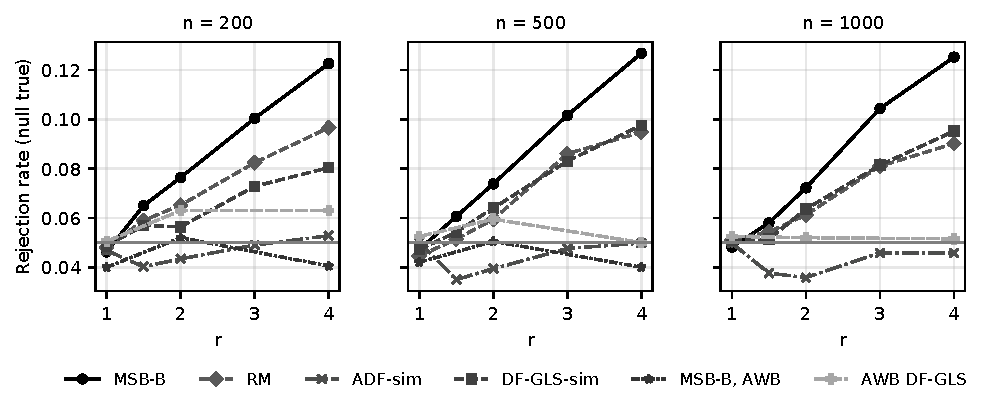
\includegraphics[width=\textwidth]{fig_dgp3_audit13q}
\caption{Rejection frequencies under a random walk with a variance break
of ratio $r$; the null is true.}
\label{fig:dgp3}
\end{figure}

\subsection*{Heavy tails and conditional heteroskedasticity}

\Cref{tab:misspec} repeats the size experiment with Student-$t$
innovations and with GARCH$(1,1)$ innovations of persistence $0.95$,
$0.98$ and $0.99$ (normal) and $0.95$ ($t(5)$), standardized to unit
unconditional variance, without recalibrating. The fourth-moment
condition holds in all four GARCH specifications. We summarize the GARCH
cells by the mean shift of each test's size relative to its own size
under Gaussian innovations at the same $n$ (\cref{fig:sizeshift}).

Under heavy tails \RMGLS{} is slightly conservative at $n = 200$ ($0.044$
and $0.043$) and within the region at larger $n$, like DF-GLS and the M
tests, while ADF and PP with asymptotic critical values over-reject.
Under GARCH its distortion lies between that of the GLS tests and that of
ADF: at $n = 200$ its mean shift is $+0.63$ points, against $+0.28$ for
DF-GLS, $+0.39$ for MZ$_t$-GLS and $+1.47$ for ADF with simulated
critical values; at $n = 1000$ the figures are $+0.33$, $+0.04$, $+0.21$
and $+0.85$. It is inside the exact region in nine of the sixteen GARCH
cells, against eleven for DF-GLS and MZ$_t$-GLS, nine for MSB-GLS, six for
ADF with simulated and four with asymptotic critical values, and two for
PP. We draw no robustness claim from these results: under conditional
heteroskedasticity \RMGLS{} behaves as a GLS-based M test does, slightly
worse than DF-GLS.

\begin{table}[t]
\centering
\caption{Size under heavy-tailed and GARCH innovations, Gaussian
calibration unchanged, $\alpha = 0.05$.}
\label{tab:misspec}
\footnotesize
\resizebox{\textwidth}{!}{%
% Generado por experiments/audit13_tables.py desde b92_theta_audit9.json (no editar a mano)
\begin{tabular}{lrccccccc}
\toprule
Innovations & $n$ & \RMGLS{} & ADF-sim & ADF & PP & DF-GLS & MZ$_t$ & MSB \\
\midrule
$t(5)$ & 200 & \textbf{0.0438} & 0.0528 & \textbf{0.0628} & \textbf{0.0584} & \textbf{0.0438} & 0.0440 & 0.0442 \\
$t(5)$ & 500 & 0.0510 & 0.0522 & 0.0552 & \textbf{0.0614} & 0.0496 & 0.0504 & 0.0502 \\
$t(5)$ & 1000 & 0.0486 & 0.0496 & 0.0500 & 0.0540 & 0.0466 & 0.0468 & 0.0488 \\
$t(3)$ & 200 & \textbf{0.0428} & 0.0520 & \textbf{0.0624} & \textbf{0.0612} & \textbf{0.0414} & \textbf{0.0422} & 0.0446 \\
$t(3)$ & 500 & 0.0502 & 0.0488 & 0.0528 & \textbf{0.0590} & 0.0520 & 0.0520 & 0.0498 \\
$t(3)$ & 1000 & 0.0470 & 0.0524 & 0.0528 & \textbf{0.0600} & 0.0502 & 0.0496 & 0.0474 \\
G 0.95, N & 200 & 0.0500 & \textbf{0.0630} & \textbf{0.0724} & \textbf{0.0736} & \textbf{0.0430} & 0.0454 & \textbf{0.0432} \\
G 0.95, N & 500 & 0.0554 & \textbf{0.0576} & \textbf{0.0612} & \textbf{0.0610} & 0.0480 & 0.0516 & 0.0504 \\
G 0.95, N & 1000 & 0.0480 & 0.0490 & 0.0494 & 0.0520 & 0.0462 & 0.0470 & 0.0496 \\
G 0.98, N & 200 & \textbf{0.0606} & 0.0536 & \textbf{0.0648} & \textbf{0.0688} & 0.0556 & \textbf{0.0572} & \textbf{0.0606} \\
G 0.98, N & 500 & \textbf{0.0576} & \textbf{0.0622} & \textbf{0.0640} & \textbf{0.0708} & 0.0514 & 0.0550 & 0.0538 \\
G 0.98, N & 1000 & 0.0514 & \textbf{0.0640} & \textbf{0.0644} & \textbf{0.0654} & 0.0484 & 0.0504 & 0.0496 \\
G 0.99, N & 200 & \textbf{0.0602} & \textbf{0.0600} & \textbf{0.0730} & \textbf{0.0736} & \textbf{0.0616} & \textbf{0.0626} & \textbf{0.0622} \\
G 0.99, N & 500 & \textbf{0.0596} & \textbf{0.0584} & \textbf{0.0620} & \textbf{0.0672} & \textbf{0.0572} & \textbf{0.0580} & \textbf{0.0588} \\
G 0.99, N & 1000 & \textbf{0.0614} & \textbf{0.0642} & \textbf{0.0654} & \textbf{0.0696} & \textbf{0.0584} & \textbf{0.0598} & \textbf{0.0626} \\
G 0.99, N & 2000 & 0.0548 & 0.0544 & 0.0544 & \textbf{0.0578} & 0.0518 & 0.0530 & 0.0540 \\
G 0.99, N & 5000 & 0.0546 & 0.0546 & 0.0546 & 0.0556 & 0.0534 & 0.0538 & 0.0538 \\
G 0.95, $t(5)$ & 200 & 0.0550 & \textbf{0.0724} & \textbf{0.0832} & \textbf{0.0784} & 0.0498 & 0.0526 & 0.0518 \\
G 0.95, $t(5)$ & 500 & \textbf{0.0604} & \textbf{0.0644} & \textbf{0.0690} & \textbf{0.0702} & \textbf{0.0582} & \textbf{0.0596} & \textbf{0.0590} \\
G 0.95, $t(5)$ & 1000 & \textbf{0.0576} & \textbf{0.0576} & \textbf{0.0580} & \textbf{0.0618} & 0.0528 & 0.0562 & \textbf{0.0566} \\
G 0.95, $t(5)$ & 2000 & 0.0560 & 0.0502 & 0.0504 & \textbf{0.0564} & 0.0516 & 0.0538 & 0.0512 \\
G 0.95, $t(5)$ & 5000 & 0.0534 & 0.0560 & \textbf{0.0566} & \textbf{0.0570} & 0.0512 & 0.0516 & 0.0496 \\
\midrule
\multicolumn{9}{l}{\emph{Mean shift relative to Gaussian size, GARCH cells, percentage points (s.e.)}}\\
\multicolumn{2}{l}{$n = 200$ (4)} & +0.63 (0.18) & +1.47 (0.19) & +1.61 (0.20) & +1.61 (0.20) & +0.28 (0.18) & +0.39 (0.18) & +0.42 (0.18) \\
\multicolumn{2}{l}{$n = 500$ (4)} & +1.12 (0.18) & +1.27 (0.18) & +1.20 (0.19) & +1.15 (0.19) & +0.84 (0.18) & +1.04 (0.18) & +0.82 (0.18) \\
\multicolumn{2}{l}{$n = 1000$ (4)} & +0.33 (0.18) & +0.85 (0.18) & +0.82 (0.18) & +0.78 (0.19) & +0.04 (0.17) & +0.21 (0.18) & +0.40 (0.18) \\
\multicolumn{2}{l}{$n = 2000$ (2)} & +0.84 (0.25) & +0.23 (0.25) & +0.24 (0.25) & +0.37 (0.26) & +0.36 (0.25) & +0.57 (0.25) & +0.59 (0.25) \\
\multicolumn{2}{l}{$n = 5000$ (2)} & +0.51 (0.25) & +0.29 (0.25) & +0.29 (0.25) & +0.22 (0.26) & +0.18 (0.25) & +0.24 (0.25) & +0.30 (0.25) \\
\bottomrule
\end{tabular}
}
\par\medskip\begin{minipage}{\textwidth}\footnotesize  5000 common paths per cell; constant case. ``G $p$, N'': GARCH(1,1)
with persistence $p$ and normal innovations; ``G 0.95, $t(5)$'':
standardized $t(5)$ innovations. DF-GLS, MZ$_t$ and MSB are the GLS
versions with simulated critical values; ADF and PP without suffix use
asymptotic critical values. Bold: outside $[0.0440, 0.0562]$. Shifts are
relative to the size of each test under Gaussian innovations on $2\times
10^4$ independent paths at the same $n$; the number of cells averaged is
in parentheses.
\end{minipage}
\end{table}

\begin{figure}[t]
\centering
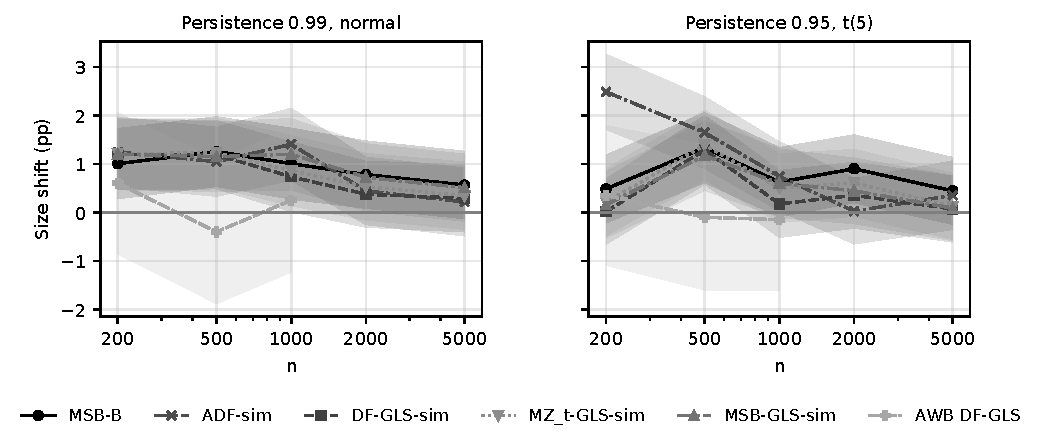
\includegraphics[width=\textwidth]{fig_size_shift_audit13q}
\caption{Shift in size under GARCH innovations relative to Gaussian
innovations, in percentage points, for the two specifications evaluated
up to $n=5000$. Bands: $\pm1.96$ standard errors.}
\label{fig:sizeshift}
\end{figure}

The sieve bootstrap (SB) and the sieve wild bootstrap (SWB) calibrations of MZ$_t$-GLS were not evaluated under variance breaks.

\FloatBarrier
\section{The smoothed family $S_\theta$}\label{supp:s5}

For a window fraction $\theta \in [0, 1/2]$ let $\tau = \mathrm{round}(\theta
n)$ and define the rolling means of the detrended series,
\begin{equation}\label{eq:rollmean}
\rmean_k = \frac{1}{\tau+1}\sum_{i=k}^{k+\tau} \uhat_i,
\qquad k = 0, 1, \dots, n - \tau,
\end{equation}
over $N_k = n - \tau + 1$ overlapping windows, and
\begin{equation}\label{eq:stat}
\Stat = \frac{\Big(N_k^{-1}\sum_{k=0}^{n-\tau}\rmean_k^{\,2}\Big)^{1/2}}
{\hacsig\, n^{1/2}}.
\end{equation}

\subsection*{The smoothing window}

The smoothed statistics $\Stat$ with $\theta > 0$ were compared with
$\theta = 0$ under a rule written before the comparison was run.
Five values $\theta \in \{0, 0.02, 0.05, 0.1, 0.2\}$ were eligible if (A1)
their size under equation~(2) of the main text lay within $0.25$ percentage points of
$0.05$ at $n \in \{200, 500, 1000\}$ in both deterministic cases, measured
on $10^5$ independent paths per cell with $\ncal = 5\times10^5$, and (A2)
their mean size distortion over sixteen GARCH cells with $n \leq 500$ was
within $0.3$ points of the best. Among eligible values, the one with the
highest mean local power at $c \in \{5, 10, 15\}$ was selected, with ties
within one point broken in favour of the larger window. All five values
were eligible, with a worst deviation from $0.05$ of $0.10$ points. Mean
local power was $0.659$, $0.654$, $0.645$, $0.631$ and $0.601$ for the five
values in increasing order; $\theta = 0$ and $\theta = 0.02$ tied, and the
rule selected $\theta = 0.02$.

The rule was amended once, and we report the amendment. A first
evaluation used $2\times10^4$ paths shared between the two deterministic
cases and $\ncal = 5\times10^4$; in it, four of the five windows failed
(A1) in a single cell, the trend case at $n=200$, by margins below
$0.001$, and so did nine of twelve comparator tests evaluated on the same
paths. A second evaluation with independent paths per case and a tenfold
larger calibration found every procedure within tolerance in that cell
(rates from $0.0494$ to $0.0503$), and the amended criterion replaced a
binomial acceptance region by the equivalence margin stated above. The
amendment was registered before the second evaluation was run.

The rule's tie-break in favour of the larger window had no stated
rationale. Its only support in the data is the GARCH criterion (A2), on
which the two windows differ by $0.01$ points, and every other comparison
favours $\theta = 0$. On the finite-sample power designs of
Section~S1 and Section~S4, $\theta = 0$ has higher power than
$\theta = 0.02$ (McNemar $p < 0.05$) in 12 of the 23
cells in which at least one of the two rejects with probability strictly
between $0$ and $0.99$, and lower power in 2, by at most
$0.4$ points; under a variance break with the null true it is less
distorted in 5 of 12 cells and more distorted in none; and under a unit
root with moving-average errors of $-0.8$ at $n = 200$ it rejects $0.420$
and $0.361$ in the constant and trend cases, against $0.531$ and $0.781$
with $\theta = 0.02$. We therefore report the statistic without a window.
This is a departure from the configuration selected by the registered
rule, not a change of the rule: the rule's output, $\theta = 0.02$, is
reported here, lies within the rule's own tie margin of $\theta = 0$, and
its results are in the supplement; \cref{tab:deviations} records the
departure and its effect on the application.

\begin{figure}[t]
\centering
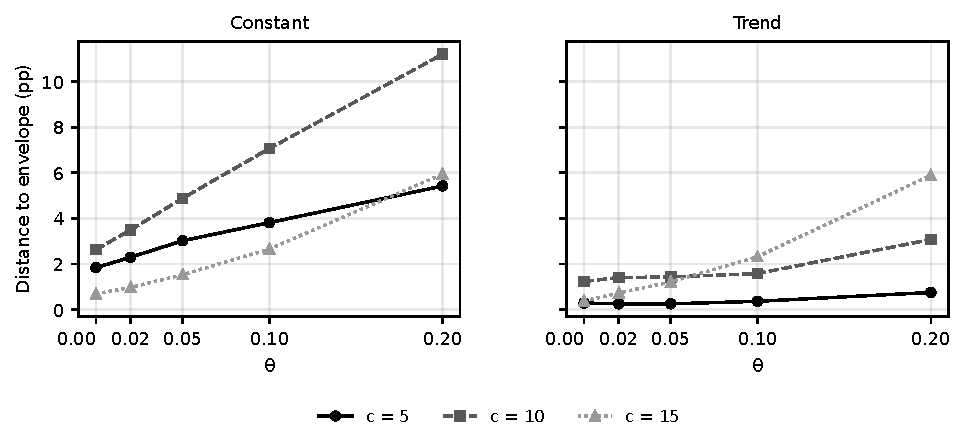
\includegraphics[width=\textwidth]{fig_theta_ladder_audit13q}
\caption{Distance to the Gaussian power envelope, in percentage points,
against the window $\theta$ of the smoothed statistic, at $c \in \{5, 10,
15\}$.}
\label{fig:thetaladder}
\end{figure}

\subsection*{Tables with $\theta = 0.02$}

RM: the centred rolling-means statistic with $\theta = 0.1$.

\begin{table}[htbp]
\centering
\caption{As \cref{tab:size}, computed with $\theta = 0.02$. Bold entries follow the rule stated in its note.}
\label{tab:size02}
\small
\begin{adjustbox}{max width=\textwidth}
% Generado por experiments/audit15_supplement.py desde tables_audit13.json (valores con theta = 0.02, disposicion del v13) (no editar a mano)
\begin{tabular}{rcc}
\toprule
$n$ & Constant & Trend \\
\midrule
60 & 0.0496 [0.0477, 0.0515] & 0.0489 [0.0471, 0.0508] \\
100 & 0.0510 [0.0491, 0.0530] & 0.0496 [0.0477, 0.0515] \\
150 & 0.0476 [0.0458, 0.0495] & 0.0506 [0.0487, 0.0525] \\
200 & 0.0501 [0.0488, 0.0515] & 0.0500 [0.0486, 0.0513] \\
500 & 0.0491 [0.0477, 0.0504] & 0.0504 [0.0491, 0.0518] \\
1000 & 0.0490 [0.0477, 0.0504] & 0.0505 [0.0492, 0.0519] \\
\bottomrule
\end{tabular}

\end{adjustbox}
\end{table}

\begin{table}[htbp]
\centering
\caption{As Table~1 of the main text, computed with $\theta = 0.02$. Bold entries follow the rule stated in its note.}
\label{tab:calib02}
\small
\begin{adjustbox}{max width=\textwidth}
% Generado por experiments/audit15_supplement.py desde tables_audit13.json (valores con theta = 0.02, disposicion del v13) (no editar a mano)
\begin{tabular}{rccccccc}
\toprule
& \multicolumn{3}{c}{$S_{0.02}$} & \multicolumn{2}{c}{DF-GLS} & \multicolumn{2}{c}{MSB-GLS}\\
\cmidrule(lr){2-4}\cmidrule(lr){5-6}\cmidrule(lr){7-8}
$n$ & $q_{0.05}(n)$ & at $q(n)$ & at $q(20\,000)$ & asy. & sim. & asy. & sim.\\
\midrule
\multicolumn{8}{l}{\emph{Constant}}\\
60 & 0.2148 & \textbf{0.0541} & \textbf{0.0785} & \textbf{0.0660} & 0.0520 & 0.0502 & 0.0503 \\
100 & 0.2218 & 0.0517 & \textbf{0.0638} & \textbf{0.0568} & 0.0520 & 0.0496 & 0.0527 \\
150 & 0.2228 & 0.0499 & \textbf{0.0592} & \textbf{0.0536} & 0.0516 & \textbf{0.0442} & 0.0486 \\
200 & 0.2243 & 0.0510 & \textbf{0.0574} & 0.0513 & 0.0503 & \textbf{0.0460} & 0.0509 \\
500 & 0.2279 & 0.0474 & 0.0491 & \textbf{0.0452} & \textbf{0.0459} & \textbf{0.0417} & 0.0471 \\
1000 & 0.2288 & 0.0517 & 0.0528 & 0.0498 & 0.0510 & \textbf{0.0461} & 0.0508 \\
2000 & 0.2287 & \textbf{0.0464} & 0.0476 & 0.0478 & 0.0481 & \textbf{0.0430} & \textbf{0.0467} \\
5000 & 0.2300 & 0.0491 & 0.0490 & 0.0498 & 0.0505 & \textbf{0.0449} & 0.0487 \\
\multicolumn{8}{l}{\emph{Trend}}\\
60 & 0.1620 & 0.0515 & 0.0524 & \textbf{0.0534} & 0.0517 & \textbf{0.0169} & 0.0513 \\
100 & 0.1649 & 0.0486 & \textbf{0.0437} & \textbf{0.0420} & 0.0496 & \textbf{0.0225} & 0.0485 \\
150 & 0.1635 & 0.0506 & 0.0480 & \textbf{0.0386} & 0.0493 & \textbf{0.0261} & 0.0504 \\
200 & 0.1627 & 0.0476 & \textbf{0.0467} & \textbf{0.0350} & 0.0474 & \textbf{0.0260} & 0.0474 \\
500 & 0.1623 & 0.0490 & 0.0495 & \textbf{0.0381} & 0.0486 & \textbf{0.0336} & 0.0484 \\
1000 & 0.1622 & 0.0513 & 0.0516 & \textbf{0.0413} & 0.0495 & \textbf{0.0394} & 0.0503 \\
2000 & 0.1620 & 0.0480 & 0.0493 & \textbf{0.0411} & 0.0484 & \textbf{0.0398} & 0.0482 \\
5000 & 0.1629 & 0.0512 & 0.0505 & \textbf{0.0440} & 0.0524 & \textbf{0.0428} & 0.0522 \\
\bottomrule
\end{tabular}

\end{adjustbox}
\end{table}

\begin{table}[htbp]
\centering
\caption{As Table~2 of the main text, computed with $\theta = 0.02$. Bold entries follow the rule stated in its note.}
\label{tab:localpower02}
\small
\begin{adjustbox}{max width=\textwidth}
% Generado por experiments/audit15_supplement.py desde tables_audit13.json (valores con theta = 0.02, disposicion del v13) (no editar a mano)
\begin{tabular}{rccccccc}
\toprule
$c$ & Envelope & $S_{0.02}$ & $\theta = 0$ & DF-GLS & MZ$_t$-GLS & MSB-GLS & MSB-GLS asy.\\
\midrule
\multicolumn{8}{l}{\emph{Constant}}\\
2 & 0.118 & 0.110 & 0.111 & 0.115 & 0.115 & 0.109 & 0.103 \\
5 & 0.313 & 0.290 & 0.295 & 0.311 & 0.312 & 0.290 & 0.274 \\
7 & 0.497 & 0.458 & 0.464 & 0.494 & 0.495 & 0.460 & 0.438 \\
10 & 0.750 & 0.716 & 0.724 & 0.751 & 0.752 & 0.720 & 0.695 \\
13.5 & 0.930 & 0.915 & 0.919 & 0.927 & 0.927 & 0.915 & 0.901 \\
15 & 0.965 & 0.955 & 0.958 & 0.962 & 0.963 & 0.955 & 0.947 \\
20 & 0.998 & 0.997 & 0.998 & 0.996 & 0.996 & 0.997 & 0.996 \\
\multicolumn{8}{l}{\emph{Trend}}\\
2 & 0.060 & 0.061 & 0.061 & 0.060 & 0.061 & 0.060 & 0.049 \\
5 & 0.115 & 0.113 & 0.112 & 0.117 & 0.116 & 0.114 & 0.093 \\
7 & 0.175 & 0.170 & 0.171 & 0.175 & 0.175 & 0.171 & 0.144 \\
10 & 0.309 & 0.295 & 0.296 & 0.307 & 0.306 & 0.297 & 0.256 \\
13.5 & 0.506 & 0.495 & 0.498 & 0.506 & 0.506 & 0.495 & 0.437 \\
15 & 0.591 & 0.584 & 0.588 & 0.591 & 0.591 & 0.582 & 0.526 \\
20 & 0.846 & 0.843 & 0.846 & 0.846 & 0.846 & 0.839 & 0.793 \\
\bottomrule
\end{tabular}

\end{adjustbox}
\end{table}

\begin{table}[htbp]
\centering
\caption{As \cref{tab:dgp1}, computed with $\theta = 0.02$. Bold entries follow the rule stated in its note.}
\label{tab:dgp102}
\small
\begin{adjustbox}{max width=\textwidth}
% Generado por experiments/audit15_supplement.py desde tables_audit13.json (valores con theta = 0.02, disposicion del v13) (no editar a mano)
\begin{tabular}{rrcccccccc}
\toprule
$\rho$ & $n$ & $S_{0.02}$ & RM & ADF & PP & DF-GLS & MZ$_t$ & MSB & $p$ \\
\midrule
0.85 & 200 & 1.000 & 0.994 & 0.958 & 0.995 & 0.953 & 0.944 & 0.941 & $<$0.001 \\
0.90 & 200 & 0.993 & 0.896 & 0.798 & 0.850 & 0.926 & 0.928 & 0.922 & $<$0.001 \\
0.93 & 200 & 0.905 & 0.647 & 0.491 & 0.538 & 0.854 & 0.856 & 0.835 & $<$0.001 \\
0.95 & 200 & 0.701 & 0.426 & 0.291 & 0.313 & 0.690 & 0.691 & 0.654 & 0.057 \\
0.97 & 200 & 0.381 & 0.233 & 0.147 & 0.150 & 0.397 & 0.393 & 0.365 & 0.003 \\
0.99 & 200 & 0.114 & 0.092 & 0.067 & 0.066 & 0.111 & 0.112 & 0.113 & 0.426 \\
0.95 & 500 & 1.000 & 0.980 & 0.939 & 0.955 & 0.992 & 0.993 & 0.992 & $<$0.001 \\
0.97 & 500 & 0.951 & 0.726 & 0.577 & 0.604 & 0.939 & 0.940 & 0.934 & 0.001 \\
0.99 & 500 & 0.296 & 0.187 & 0.119 & 0.127 & 0.316 & 0.313 & 0.295 & $<$0.001 \\
0.99 & 1000 & 0.729 & 0.434 & 0.303 & 0.318 & 0.755 & 0.755 & 0.728 & $<$0.001 \\
\bottomrule
\end{tabular}

\end{adjustbox}
\end{table}

\begin{table}[htbp]
\centering
\caption{As \cref{tab:ctpower}, computed with $\theta = 0.02$. Bold entries follow the rule stated in its note.}
\label{tab:ctpower02}
\small
\begin{adjustbox}{max width=\textwidth}
% Generado por experiments/audit15_supplement.py desde tables_audit13.json (valores con theta = 0.02, disposicion del v13) (no editar a mano)
\begin{tabular}{rrcccccccc}
\toprule
$\rho$ & $n$ & $S_{0.02}$ & RM & ADF & PP & DF-GLS & MZ$_t$ & MSB & $p$ \\
\midrule
0.90 & 200 & 0.823 & 0.740 & 0.556 & 0.630 & 0.720 & 0.742 & 0.734 & $<$0.001 \\
0.95 & 200 & 0.297 & 0.257 & 0.175 & 0.189 & 0.290 & 0.290 & 0.284 & 0.150 \\
0.97 & 200 & 0.133 & 0.122 & 0.098 & 0.096 & 0.130 & 0.132 & 0.130 & 0.450 \\
0.99 & 200 & 0.062 & 0.060 & 0.058 & 0.060 & 0.062 & 0.064 & 0.062 & 1.000 \\
0.95 & 500 & 0.958 & 0.913 & 0.782 & 0.815 & 0.899 & 0.911 & 0.910 & $<$0.001 \\
0.97 & 500 & 0.586 & 0.515 & 0.355 & 0.380 & 0.575 & 0.578 & 0.563 & 0.030 \\
0.99 & 500 & 0.099 & 0.089 & 0.072 & 0.075 & 0.102 & 0.103 & 0.100 & 0.289 \\
0.97 & 1000 & 0.994 & 0.977 & 0.913 & 0.923 & 0.975 & 0.980 & 0.980 & $<$0.001 \\
0.99 & 1000 & 0.304 & 0.270 & 0.195 & 0.198 & 0.304 & 0.305 & 0.303 & 1.000 \\
\bottomrule
\end{tabular}

\end{adjustbox}
\end{table}

\begin{table}[htbp]
\centering
\caption{As \cref{tab:dgp2}, computed with $\theta = 0.02$. Bold entries follow the rule stated in its note.}
\label{tab:dgp202}
\small
\begin{adjustbox}{max width=\textwidth}
% Generado por experiments/audit15_supplement.py desde tables_audit13.json (valores con theta = 0.02, disposicion del v13) (no editar a mano)
\begin{tabular}{r r c c c c c c c c c }
\toprule
$\delta$ & $n$ & $S_{0.02}$ ($\theta = 0.02$) & RM & ADF-sim & PP-sim & DF-GLS-sim & MZ$_t$-GLS-sim & MSB-GLS-sim & ZA & McNemar $p$ \\
\midrule
0 & 200 & 0.706 & 0.432 & 0.299 & 0.322 & 0.695 & 0.689 & 0.658 & 0.119 & 0.057 \\
0 & 500 & 1.000 & 0.980 & 0.938 & 0.949 & 0.994 & 0.995 & 0.994 & 0.454 & $<$0.001 \\
0 & 1000 & 1.000 & 1.000 & 1.000 & 1.000 & 1.000 & 1.000 & 1.000 & 0.970 & 1.000 \\
\addlinespace
0.5 & 200 & 0.635 & 0.396 & 0.269 & 0.290 & 0.620 & 0.613 & 0.594 & 0.119 & 0.017 \\
0.5 & 500 & 1.000 & 0.959 & 0.903 & 0.914 & 0.983 & 0.983 & 0.987 & 0.456 & $<$0.001 \\
0.5 & 1000 & 1.000 & 1.000 & 1.000 & 1.000 & 1.000 & 1.000 & 1.000 & 0.971 & 1.000 \\
\addlinespace
1 & 200 & 0.474 & 0.288 & 0.196 & 0.198 & 0.445 & 0.444 & 0.439 & 0.124 & $<$0.001 \\
1 & 500 & 0.990 & 0.865 & 0.784 & 0.766 & 0.931 & 0.935 & 0.941 & 0.439 & $<$0.001 \\
1 & 1000 & 1.000 & 1.000 & 0.995 & 1.000 & 0.997 & 0.997 & 0.998 & 0.966 & $<$0.001 \\
\addlinespace
2 & 200 & 0.094 & 0.080 & 0.053 & 0.048 & 0.083 & 0.083 & 0.093 & 0.104 & 0.002 \\
2 & 500 & 0.573 & 0.329 & 0.266 & 0.212 & 0.441 & 0.442 & 0.479 & 0.397 & $<$0.001 \\
2 & 1000 & 1.000 & 0.953 & 0.915 & 0.857 & 0.870 & 0.882 & 0.900 & 0.962 & $<$0.001 \\
\addlinespace
3 & 200 & 0.004 & 0.006 & 0.004 & 0.003 & 0.001 & 0.001 & 0.005 & 0.088 & 0.017 \\
3 & 500 & 0.024 & 0.018 & 0.015 & 0.008 & 0.017 & 0.017 & 0.023 & 0.378 & $<$0.001 \\
3 & 1000 & 0.637 & 0.279 & 0.328 & 0.127 & 0.376 & 0.378 & 0.456 & 0.954 & $<$0.001 \\
\addlinespace
5 & 200 & 0.000 & 0.000 & 0.000 & 0.000 & 0.000 & 0.000 & 0.000 & 0.092 & 1.000 \\
5 & 500 & 0.000 & 0.000 & 0.000 & 0.000 & 0.000 & 0.000 & 0.000 & 0.497 & 1.000 \\
5 & 1000 & 0.000 & 0.000 & 0.000 & 0.000 & 0.000 & 0.000 & 0.000 & 0.986 & 1.000 \\
\bottomrule
\end{tabular}

\end{adjustbox}
\end{table}

\begin{table}[htbp]
\centering
\caption{As \cref{tab:dgp3}, computed with $\theta = 0.02$. Bold entries follow the rule stated in its note.}
\label{tab:dgp302}
\small
\begin{adjustbox}{max width=\textwidth}
% Generado por experiments/audit15_supplement.py desde tables_audit13.json (valores con theta = 0.02, disposicion del v13) (no editar a mano)
\begin{tabular}{rrccccccc}
\toprule
$r$ & $n$ & $S_{0.02}$ & RM & ADF & PP & DF-GLS & MZ$_t$ & MSB \\
\midrule
1 & 200 & 0.048 & 0.048 & 0.047 & \textbf{0.041} & 0.049 & 0.047 & 0.047 \\
1.5 & 200 & \textbf{0.065} & \textbf{0.059} & \textbf{0.040} & \textbf{0.041} & \textbf{0.057} & \textbf{0.063} & \textbf{0.064} \\
2 & 200 & \textbf{0.078} & \textbf{0.065} & \textbf{0.043} & \textbf{0.038} & \textbf{0.056} & \textbf{0.070} & \textbf{0.080} \\
3 & 200 & \textbf{0.103} & \textbf{0.082} & 0.049 & \textbf{0.038} & \textbf{0.073} & \textbf{0.099} & \textbf{0.116} \\
4 & 200 & \textbf{0.128} & \textbf{0.097} & 0.053 & 0.047 & \textbf{0.080} & \textbf{0.117} & \textbf{0.130} \\
2 & 500 & \textbf{0.074} & \textbf{0.059} & \textbf{0.039} & \textbf{0.036} & \textbf{0.064} & \textbf{0.071} & \textbf{0.078} \\
4 & 500 & \textbf{0.131} & \textbf{0.095} & 0.050 & 0.050 & \textbf{0.098} & \textbf{0.119} & \textbf{0.135} \\
2 & 1000 & \textbf{0.073} & \textbf{0.061} & \textbf{0.036} & \textbf{0.037} & \textbf{0.064} & \textbf{0.067} & \textbf{0.074} \\
4 & 1000 & \textbf{0.127} & \textbf{0.090} & 0.046 & 0.044 & \textbf{0.095} & \textbf{0.109} & \textbf{0.131} \\
\bottomrule
\end{tabular}

\end{adjustbox}
\end{table}

\begin{table}[htbp]
\centering
\caption{As \cref{tab:misspec}, computed with $\theta = 0.02$. Bold entries follow the rule stated in its note.}
\label{tab:misspec02}
\small
\begin{adjustbox}{max width=\textwidth}
% Generado por experiments/audit15_supplement.py desde tables_audit13.json (valores con theta = 0.02, disposicion del v13) (no editar a mano)
\begin{tabular}{lrccccccc}
\toprule
Innovations & $n$ & $S_{0.02}$ & ADF-sim & ADF & PP & DF-GLS & MZ$_t$ & MSB \\
\midrule
$t(5)$ & 200 & \textbf{0.0430} & 0.0528 & \textbf{0.0628} & \textbf{0.0584} & \textbf{0.0438} & 0.0440 & 0.0442 \\
$t(5)$ & 500 & 0.0520 & 0.0522 & 0.0552 & \textbf{0.0614} & 0.0496 & 0.0504 & 0.0502 \\
$t(5)$ & 1000 & 0.0488 & 0.0496 & 0.0500 & 0.0540 & 0.0466 & 0.0468 & 0.0488 \\
$t(3)$ & 200 & \textbf{0.0422} & 0.0520 & \textbf{0.0624} & \textbf{0.0612} & \textbf{0.0414} & \textbf{0.0422} & 0.0446 \\
$t(3)$ & 500 & 0.0512 & 0.0488 & 0.0528 & \textbf{0.0590} & 0.0520 & 0.0520 & 0.0498 \\
$t(3)$ & 1000 & 0.0472 & 0.0524 & 0.0528 & \textbf{0.0600} & 0.0502 & 0.0496 & 0.0474 \\
G 0.95, normal & 200 & 0.0492 & \textbf{0.0630} & \textbf{0.0724} & \textbf{0.0736} & \textbf{0.0430} & 0.0454 & \textbf{0.0432} \\
G 0.95, normal & 500 & 0.0552 & \textbf{0.0576} & \textbf{0.0612} & \textbf{0.0610} & 0.0480 & 0.0516 & 0.0504 \\
G 0.95, normal & 1000 & 0.0494 & 0.0490 & 0.0494 & 0.0520 & 0.0462 & 0.0470 & 0.0496 \\
G 0.98, normal & 200 & \textbf{0.0608} & 0.0536 & \textbf{0.0648} & \textbf{0.0688} & 0.0556 & \textbf{0.0572} & \textbf{0.0606} \\
G 0.98, normal & 500 & \textbf{0.0580} & \textbf{0.0622} & \textbf{0.0640} & \textbf{0.0708} & 0.0514 & 0.0550 & 0.0538 \\
G 0.98, normal & 1000 & 0.0522 & \textbf{0.0640} & \textbf{0.0644} & \textbf{0.0654} & 0.0484 & 0.0504 & 0.0496 \\
G 0.99, normal & 200 & \textbf{0.0594} & \textbf{0.0600} & \textbf{0.0730} & \textbf{0.0736} & \textbf{0.0616} & \textbf{0.0626} & \textbf{0.0622} \\
G 0.99, normal & 500 & \textbf{0.0602} & \textbf{0.0584} & \textbf{0.0620} & \textbf{0.0672} & \textbf{0.0572} & \textbf{0.0580} & \textbf{0.0588} \\
G 0.99, normal & 1000 & \textbf{0.0628} & \textbf{0.0642} & \textbf{0.0654} & \textbf{0.0696} & \textbf{0.0584} & \textbf{0.0598} & \textbf{0.0626} \\
G 0.99, normal & 2000 & 0.0552 & 0.0544 & 0.0544 & \textbf{0.0578} & 0.0518 & 0.0530 & 0.0540 \\
G 0.99, normal & 5000 & 0.0552 & 0.0546 & 0.0546 & 0.0556 & 0.0534 & 0.0538 & 0.0538 \\
G 0.95, $t(5)$ & 200 & 0.0560 & \textbf{0.0724} & \textbf{0.0832} & \textbf{0.0784} & 0.0498 & 0.0526 & 0.0518 \\
G 0.95, $t(5)$ & 500 & \textbf{0.0608} & \textbf{0.0644} & \textbf{0.0690} & \textbf{0.0702} & \textbf{0.0582} & \textbf{0.0596} & \textbf{0.0590} \\
G 0.95, $t(5)$ & 1000 & \textbf{0.0576} & \textbf{0.0576} & \textbf{0.0580} & \textbf{0.0618} & 0.0528 & 0.0562 & \textbf{0.0566} \\
G 0.95, $t(5)$ & 2000 & 0.0560 & 0.0502 & 0.0504 & \textbf{0.0564} & 0.0516 & 0.0538 & 0.0512 \\
G 0.95, $t(5)$ & 5000 & 0.0528 & 0.0560 & \textbf{0.0566} & \textbf{0.0570} & 0.0512 & 0.0516 & 0.0496 \\
\midrule
\multicolumn{9}{l}{\emph{Mean shift relative to Gaussian size, GARCH cells, percentage points (s.e.)}}\\
\multicolumn{2}{l}{$n = 200$ (4)} & +0.63 (0.18) & +1.47 (0.19) & +1.61 (0.20) & +1.61 (0.20) & +0.28 (0.18) & +0.39 (0.18) & +0.42 (0.18) \\
\multicolumn{2}{l}{$n = 500$ (4)} & +1.10 (0.18) & +1.27 (0.18) & +1.20 (0.19) & +1.15 (0.19) & +0.84 (0.18) & +1.04 (0.18) & +0.82 (0.18) \\
\multicolumn{2}{l}{$n = 1000$ (4)} & +0.36 (0.18) & +0.85 (0.18) & +0.82 (0.18) & +0.78 (0.19) & +0.04 (0.17) & +0.21 (0.18) & +0.40 (0.18) \\
\multicolumn{2}{l}{$n = 2000$ (2)} & +0.92 (0.25) & +0.23 (0.25) & +0.24 (0.25) & +0.37 (0.26) & +0.36 (0.25) & +0.57 (0.25) & +0.59 (0.25) \\
\multicolumn{2}{l}{$n = 5000$ (2)} & +0.48 (0.25) & +0.29 (0.25) & +0.29 (0.25) & +0.22 (0.26) & +0.18 (0.25) & +0.24 (0.25) & +0.30 (0.25) \\
\bottomrule
\end{tabular}

\end{adjustbox}
\end{table}

\begin{table}[htbp]
\centering
\caption{As \cref{tab:awb}, computed with $\theta = 0.02$. Bold entries follow the rule stated in its note.}
\label{tab:awb02}
\small
\begin{adjustbox}{max width=\textwidth}
% Generado por experiments/audit15_supplement.py desde tables_audit13.json (valores con theta = 0.02, disposicion del v13) (no editar a mano)
\begin{tabular}{llcccc}
\toprule
Design & $n$ & AWB & Simulated & McNemar $p$ & Power loss (pp)\\
\midrule
Random walk, $r = 1$ & 200 & 0.042 & 0.043 & 0.804 &  \\
Random walk, $r = 1$ & 500 & 0.047 & 0.051 & 0.134 &  \\
Random walk, $r = 2$ & 200 & 0.054 & \textbf{0.082} & $<$0.001 &  \\
Random walk, $r = 2$ & 500 & 0.057 & \textbf{0.087} & $<$0.001 &  \\
Random walk, $r = 4$ & 200 & \textbf{0.040} & \textbf{0.124} & $<$0.001 &  \\
Random walk, $r = 4$ & 500 & \textbf{0.040} & \textbf{0.118} & $<$0.001 &  \\
GARCH 0.95, normal & 200 & 0.042 & 0.051 & 0.006 &  \\
GARCH 0.98, normal & 200 & 0.053 & 0.059 & 0.035 &  \\
GARCH 0.99, normal & 200 & 0.056 & 0.059 & 0.418 &  \\
GARCH 0.95, $t(5)$ & 200 & 0.045 & 0.052 & 0.007 &  \\
Gaussian random walk & 200 & 0.052 & 0.053 & 0.851 &  \\
Gaussian random walk & 500 & 0.043 & 0.047 & 0.118 &  \\
AR$(0.95)$ & 200 & 0.667 & 0.697 & $<$0.001 & 3.0 \\
AR$(0.95)$ & 500 & 1.000 & 1.000 & 1.000 & 0.0 \\
AR$(0.99)$ & 200 & 0.092 & 0.102 & 0.018 & 1.0 \\
AR$(0.99)$ & 500 & 0.296 & 0.309 & 0.011 & 1.3 \\
\bottomrule
\end{tabular}

\end{adjustbox}
\end{table}

\begin{table}[htbp]
\centering
\caption{As \cref{tab:dgp5}, computed with $\theta = 0.02$. Bold entries follow the rule stated in its note.}
\label{tab:dgp502}
\small
\begin{adjustbox}{max width=\textwidth}
% Generado por experiments/audit15_supplement.py desde tables_audit13.json (valores con theta = 0.02, disposicion del v13) (no editar a mano)
\begin{tabular}{rrccccc}
\toprule
$\rho$ & $r$ & $S_{0.02}$ & Two-channel & Union & Bootstrap DF-GLS & $g_2$ share \\
\midrule
0.93 & 1 & 0.912 & 0.658 & 0.807 & 0.924 & 0.48\% \\
0.93 & 1.25 & 0.904 & 0.658 & 0.856 & 0.906 & 0.54\% \\
0.93 & 1.5 & 0.916 & 0.685 & 0.970 & 0.889 & 0.65\% \\
0.93 & 2$^\dagger$ & 0.912 & 0.677 & 0.999 & 0.850 & 0.96\% \\
0.93 & 3$^\dagger$ & 0.894 & 0.697 & 1.000 & 0.768 & 1.38\% \\
0.93 & 4 & 0.882 & 0.687 & 1.000 & 0.704 & 1.65\% \\
0.95 & 1 & 0.694 & 0.449 & 0.540 & 0.730 & 0.43\% \\
0.95 & 1.25 & 0.717 & 0.438 & 0.684 & 0.707 & 0.47\% \\
0.95 & 1.5 & 0.712 & 0.427 & 0.926 & 0.685 & 0.53\% \\
0.95 & 2$^\dagger$ & 0.735 & 0.498 & 0.999 & 0.639 & 0.79\% \\
0.95 & 3$^\dagger$ & 0.723 & 0.470 & 1.000 & 0.523 & 1.14\% \\
0.95 & 4 & 0.722 & 0.496 & 1.000 & 0.501 & 1.38\% \\
\bottomrule
\end{tabular}

\end{adjustbox}
\par\medskip\begin{minipage}{\textwidth}\footnotesize
% Generado por experiments/audit15_supplement.py desde texto de las marcas del v13 (tab:dgp5) (no editar a mano)
$^\dagger$Registered interior.

\end{minipage}
\end{table}

\begin{table}[htbp]
\centering
\caption{As \cref{tab:fp}, computed with $\theta = 0.02$. Bold entries follow the rule stated in its note.}
\label{tab:fp02}
\small
\begin{adjustbox}{max width=\textwidth}
% Generado por experiments/audit15_supplement.py desde tables_audit13.json (valores con theta = 0.02, disposicion del v13) (no editar a mano)
\begin{tabular}{lccccccc}
\toprule
& \multicolumn{4}{c}{Nominal level} & \multicolumn{3}{c}{Common rate}\\
\cmidrule(lr){2-5}\cmidrule(lr){6-8}
Test & FP mean & FP max & Detections & Latency & Episodes & Run & Latency$^c$\\
\midrule
$S_{0.02}$ & 0.0229 & 0.212 & 17 & 29.6 & 33 & 144.6 & 102.5 \\
$S_{0.02}$, AWB & 0.0220 & 0.229 & 15 & 32.8 & 41 & 131.9 & 105.1 \\
Registered statistic & 0.0277 & 0.437 & 13 & 33.8 & 11 & 199.6 & 109.3 \\
ADF & 0.0535 & 0.269 & 26 & 33.7 & 49 & 120.9 & 107.4 \\
PP & 0.0532 & 0.380 & 23 & 33.4 & 55 & 113.9 & 109.4 \\
DF-GLS (AIC) & 0.0323 & 0.269 & 28 & 30.6 & 33 & 144.9 & 93.6 \\
DF-GLS (MAIC) & 0.0210 & 0.273 & 23 & 33.8 & 35 & 141.2 & 96.8 \\
MZ$_t$-GLS & 0.0173 & 0.237 & 36 & 22.1 & 38 & 136.3 & 79.7 \\
KPSS$^a$ & 0.9354 & 1.000 & 87 & 1.2 & -- & -- & -- \\
\bottomrule
\end{tabular}

\end{adjustbox}
\par\medskip\begin{minipage}{\textwidth}\footnotesize
% Generado por experiments/audit15_supplement.py desde texto de las marcas del v13 (tab:fp) (no editar a mano)
$^a$KPSS tests the null of stationarity; log-prices are nonstationary, so its near-universal rejection is correct behaviour and disqualifies it as a calm-period monitor. Latency$^c$ is censored at 120 days over all 88 event cells.

\end{minipage}
\end{table}

\FloatBarrier
\section{The two-channel construction and other negative results}\label{supp:s6}

\subsection*{A pre-registered test of a two-channel extension}

The statistic was originally one channel of a two-channel construction
whose second channel measured the variability of rolling variances. The
rationale for such a construction cannot be that it detects two kinds of
departure, since two separate tests also do; it must be that a single
statistic avoids the multiplicity cost of running two. We registered,
before running it, an experiment designed to test that claim: a
stationary AR$(1)$ with $\rho \in \{0.90, 0.93, 0.95\}$ carrying a
mid-sample variance break of ratio $r \in \{1, 2, 3, 4\}$, $n = 200$,
2000 paths, every procedure calibrated to exact size $0.05$ under
equation~(2) of the main text. The comparator was the union of the wild-bootstrap
DF-GLS and the variance-break statistic $\kappa_2$ of
\citet{sanso2004testing}, calibrated jointly. The registered prediction
was that the two-channel statistic would exceed the union in the interior
of the grid, $r \in \{2, 3\}$; the registered falsification condition was
failure to do so anywhere in that interior.

The prediction failed in every interior cell (\cref{tab:dgp5}). The union
rejects with probability $0.9985$ to $1.0000$ there, against $0.47$ to
$0.90$ for the two-channel statistic. The variance channel carried
between $0.4$ and $2.0$ per cent of the squared statistic in this design
at $n = 200$,
and its power was flat in $r$. The failure has a structural reason that we
did not recognize when registering the prediction: the test rejects in
the lower tail, and a variance break raises the variance channel, so any
weight on that channel moves the statistic away from rejection when a
break is present. No normalization of the channels can turn a
second-moment departure into a route to rejection.

The one-channel \RMGLS{} changes the magnitudes but not the verdict. It
exceeds the two-channel statistic by $19$ to $29$ points in the rows of
\cref{tab:dgp5} and by at least $7.9$ points in every cell of the full grid,
exceeds the bootstrap DF-GLS for $r \geq 1.5$, and exceeds the union at $r
\leq 1.25$, where the variance break is too weak for $\kappa_2$; in the
registered interior the union still dominates it.

\begin{table}[t]
\centering
\caption{Pre-registered experiment: stationary AR$(1)$ with a mid-sample
variance break of ratio $r$, $n=200$, power at equalized size.}
\label{tab:dgp5}
\begin{threeparttable}
\small
% Generado por experiments/audit15_supplement.py desde e_dgp5_audit13.json (no editar a mano)
\begin{tabular}{rrccccc}
\toprule
$\rho$ & $r$ & \RMGLS{} & Two-channel & Union & Bootstrap DF-GLS & $g_2$ share \\
\midrule
0.90 & 1 & 0.992 & 0.893 & 0.970 & 0.997 & 0.55\% \\
0.90 & 1.1 & 0.991 & 0.912 & 0.968 & 0.992 & 0.56\% \\
0.90 & 1.25 & 0.991 & 0.904 & 0.978 & 0.989 & 0.63\% \\
0.90 & 1.5 & 0.992 & 0.890 & 0.992 & 0.985 & 0.76\% \\
0.90 & 2 & 0.985 & 0.889 & 1.000 & 0.968 & 1.12\% \\
0.90 & 3 & 0.987 & 0.903 & 1.000 & 0.933 & 1.68\% \\
0.90 & 4 & 0.974 & 0.877 & 1.000 & 0.908 & 1.98\% \\
\addlinespace
0.93 & 1 & 0.914 & 0.658 & 0.807 & 0.924 & 0.48\% \\
0.93 & 1.1 & 0.912 & 0.686 & 0.813 & 0.921 & 0.49\% \\
0.93 & 1.25 & 0.905 & 0.658 & 0.856 & 0.906 & 0.54\% \\
0.93 & 1.5 & 0.916 & 0.685 & 0.970 & 0.889 & 0.65\% \\
0.93 & 2 & 0.913 & 0.677 & 0.999 & 0.850 & 0.96\% \\
0.93 & 3 & 0.894 & 0.697 & 1.000 & 0.768 & 1.38\% \\
0.93 & 4 & 0.881 & 0.687 & 1.000 & 0.704 & 1.65\% \\
\addlinespace
0.95 & 1 & 0.702 & 0.449 & 0.540 & 0.730 & 0.43\% \\
0.95 & 1.1 & 0.721 & 0.448 & 0.571 & 0.737 & 0.44\% \\
0.95 & 1.25 & 0.721 & 0.438 & 0.684 & 0.707 & 0.47\% \\
0.95 & 1.5 & 0.713 & 0.427 & 0.926 & 0.685 & 0.53\% \\
0.95 & 2 & 0.734 & 0.498 & 0.999 & 0.639 & 0.79\% \\
0.95 & 3 & 0.721 & 0.470 & 1.000 & 0.523 & 1.14\% \\
0.95 & 4 & 0.723 & 0.496 & 1.000 & 0.501 & 1.38\% \\
\bottomrule
\end{tabular}

\begin{tablenotes}\footnotesize
\item ``Two-channel'': the original
construction with fixed weight $0.5$ on each channel; $g_2$ share: median
share of the variance channel in its squared value. The union of the
wild-bootstrap DF-GLS and $\kappa_2$ is calibrated jointly
($\alpha^\ast = 0.0256$).
\end{tablenotes}
\end{threeparttable}
\end{table}

\subsection*{Other negative results}

Three further elements of the original construction were measured and
removed. First, the variance channel is inert as well as unhelpful:
dropping it changes size by at most $0.1$ points in any of the null
cells examined under Gaussian, heavy-tailed and GARCH innovations. Second, a
signal-proportional weight between the two channels concentrated at zero
under the null (mean $0.003$) and handed control to the mean channel;
rebalancing the channels to a common scale lowered power by $14$ to $28$
points. Third, measuring the rolling means from their own average rather
than from the GLS anchor costs $24.8$ points of local power at $c = 10$,
measured with $\theta = 0.1$; the centered statistic lies $33.4$ points
below the envelope there. \Cref{tab:negvariance,tab:negweight,tab:negrebal,tab:neganchor} report these experiments in full.

\begin{table}[htbp]
\centering
\caption{The variance channel: size with one and with two channels.}
\label{tab:negvariance}
\small
\begin{adjustbox}{max width=\textwidth}
% Generado por experiments/audit15_supplement.py desde b2_size_audit8.json (B2a) (no editar a mano)
\begin{tabular}{lcccc}
\toprule
Cell & One channel & Two channels ($R = 0.5$) & $\Delta$ (pp) & McNemar $p$ \\
\midrule
gauss\_n60 & 0.0330 & 0.0326 & 0.04 & 0.625 \\
gauss\_n100 & 0.0398 & 0.0396 & 0.02 & 1.000 \\
gauss\_n150 & 0.0398 & 0.0396 & 0.02 & 1.000 \\
gauss\_n200 & 0.0364 & 0.0366 & $-$0.02 & 1.000 \\
gauss\_n500 & 0.0460 & 0.0456 & 0.04 & 0.500 \\
gauss\_n1000 & 0.0500 & 0.0502 & $-$0.02 & 1.000 \\
garch\_base\_n200 & 0.0490 & 0.0488 & 0.02 & 1.000 \\
garch\_p095\_t5\_n200 & 0.0528 & 0.0522 & 0.06 & 0.375 \\
garch\_p098\_n200 & 0.0462 & 0.0460 & 0.02 & 1.000 \\
garch\_p099\_n200 & 0.0494 & 0.0494 & 0.00 & 1.000 \\
heavy\_t3\_n200 & 0.0408 & 0.0404 & 0.04 & 0.500 \\
heavy\_t5\_n200 & 0.0364 & 0.0368 & $-$0.04 & 0.625 \\
garch\_base\_n500 & 0.0540 & 0.0538 & 0.02 & 1.000 \\
garch\_p095\_t5\_n500 & 0.0602 & 0.0600 & 0.02 & 1.000 \\
garch\_p098\_n500 & 0.0560 & 0.0562 & $-$0.02 & 1.000 \\
garch\_p099\_n500 & 0.0512 & 0.0508 & 0.04 & 0.500 \\
heavy\_t3\_n500 & 0.0466 & 0.0464 & 0.02 & 1.000 \\
heavy\_t5\_n500 & 0.0454 & 0.0456 & $-$0.02 & 1.000 \\
garch\_base\_n1000 & 0.0526 & 0.0524 & 0.02 & 1.000 \\
garch\_p095\_t5\_n1000 & 0.0606 & 0.0596 & 0.10 & 0.062 \\
garch\_p098\_n1000 & 0.0592 & 0.0588 & 0.04 & 0.500 \\
garch\_p099\_n1000 & 0.0620 & 0.0618 & 0.02 & 1.000 \\
heavy\_t3\_n1000 & 0.0538 & 0.0530 & 0.08 & 0.125 \\
heavy\_t5\_n1000 & 0.0518 & 0.0518 & 0.00 & 1.000 \\
garch\_p095\_t5\_n2000 & 0.0490 & 0.0486 & 0.04 & 0.500 \\
garch\_p099\_n2000 & 0.0548 & 0.0546 & 0.02 & 1.000 \\
garch\_p095\_t5\_n5000 & 0.0534 & 0.0532 & 0.02 & 1.000 \\
garch\_p099\_n5000 & 0.0562 & 0.0566 & $-$0.04 & 0.625 \\
\bottomrule
\end{tabular}

\end{adjustbox}
\end{table}

\begin{table}[htbp]
\centering
\caption{Distribution of the signal-proportional weight under the null.}
\label{tab:negweight}
\small
\begin{adjustbox}{max width=\textwidth}
% Generado por experiments/audit15_supplement.py desde rhat_distribution_audit5b.json (no editar a mano)
\begin{tabular}{llcccc}
\toprule
Standardization & Scenario & Mean & Median & $q_{0.05}$ & $q_{0.95}$ \\
\midrule
$\sigma$ known & $H_0$, $n = 200$ & 0.0027 & 0.0018 & 0.0004 & 0.0079 \\
$\sigma$ known & $H_0$, $n = 500$ & 0.0026 & 0.0018 & 0.0004 & 0.0075 \\
$\sigma$ known & $H_0$, $n = 1000$ & 0.0025 & 0.0018 & 0.0004 & 0.0070 \\
$\sigma$ known & DGP 3, $r = 4$, $n = 1000$ & 0.0574 & 0.0398 & 0.0091 & 0.1638 \\
$\sigma$ known & DGP 4, $r = 3$, $n = 500$ & 0.1600 & 0.1479 & 0.0695 & 0.2934 \\
\addlinespace
HAC, pilot $\alpha(1)$ & $H_0$, $n = 200$ & 0.0027 & 0.0019 & 0.0005 & 0.0077 \\
HAC, pilot $\alpha(1)$ & $H_0$, $n = 500$ & 0.0026 & 0.0018 & 0.0004 & 0.0074 \\
HAC, pilot $\alpha(1)$ & $H_0$, $n = 1000$ & 0.0025 & 0.0018 & 0.0004 & 0.0071 \\
HAC, pilot $\alpha(1)$ & DGP 3, $r = 4$, $n = 1000$ & 0.0075 & 0.0049 & 0.0011 & 0.0228 \\
HAC, pilot $\alpha(1)$ & DGP 4, $r = 3$, $n = 500$ & 0.0969 & 0.0882 & 0.0418 & 0.1798 \\
\addlinespace
HAC, pilot $\alpha(2)$ & $H_0$, $n = 200$ & 0.0027 & 0.0019 & 0.0005 & 0.0076 \\
HAC, pilot $\alpha(2)$ & $H_0$, $n = 500$ & 0.0026 & 0.0018 & 0.0004 & 0.0074 \\
HAC, pilot $\alpha(2)$ & $H_0$, $n = 1000$ & 0.0025 & 0.0018 & 0.0004 & 0.0071 \\
HAC, pilot $\alpha(2)$ & DGP 3, $r = 4$, $n = 1000$ & 0.0075 & 0.0049 & 0.0011 & 0.0227 \\
HAC, pilot $\alpha(2)$ & DGP 4, $r = 3$, $n = 500$ & 0.0782 & 0.0708 & 0.0333 & 0.1464 \\
\bottomrule
\end{tabular}

\end{adjustbox}
\end{table}

\begin{table}[htbp]
\centering
\caption{Power of the adaptive and rebalanced combinations.}
\label{tab:negrebal}
\small
\begin{adjustbox}{max width=\textwidth}
% Generado por experiments/audit15_supplement.py desde adaptive_size_power_audit5b.json (no editar a mano)
\begin{tabular}{llccc}
\toprule
Configuration & Cell & Adaptive & Rebalanced & Difference (pp) \\
\midrule
$\sigma$ known, $\ncal = 10^{4}$ & $\rho = 0.95$, $n = 200$ & 0.4030 & 0.2986 & 10.44 \\
$\sigma$ known, $\ncal = 10^{4}$ & $\rho = 0.97$, $n = 500$ & 0.7236 & 0.4738 & 24.98 \\
$\sigma$ known, $\ncal = 10^{4}$ & $\rho = 0.99$, $n = 1000$ & 0.4446 & 0.3142 & 13.04 \\
\addlinespace
HAC, pilot $\alpha(1)$, $\ncal = 10^{4}$ & $\rho = 0.95$, $n = 200$ & 0.3762 & 0.2252 & 15.10 \\
HAC, pilot $\alpha(1)$, $\ncal = 10^{4}$ & $\rho = 0.97$, $n = 500$ & 0.7108 & 0.4388 & 27.20 \\
HAC, pilot $\alpha(1)$, $\ncal = 10^{4}$ & $\rho = 0.99$, $n = 1000$ & 0.4434 & 0.3002 & 14.32 \\
\addlinespace
HAC, pilot $\alpha(2)$, $\ncal = 10^{4}$ & $\rho = 0.95$, $n = 200$ & 0.3790 & 0.2304 & 14.86 \\
HAC, pilot $\alpha(2)$, $\ncal = 10^{4}$ & $\rho = 0.97$, $n = 500$ & 0.7130 & 0.4408 & 27.22 \\
HAC, pilot $\alpha(2)$, $\ncal = 10^{4}$ & $\rho = 0.99$, $n = 1000$ & 0.4436 & 0.3004 & 14.32 \\
\addlinespace
$\sigma$ known, $\ncal = 5\times10^{4}$ & $\rho = 0.95$, $n = 200$ & 0.4104 & 0.3010 & 10.94 \\
$\sigma$ known, $\ncal = 5\times10^{4}$ & $\rho = 0.97$, $n = 500$ & 0.7214 & 0.4670 & 25.44 \\
$\sigma$ known, $\ncal = 5\times10^{4}$ & $\rho = 0.99$, $n = 1000$ & 0.4486 & 0.3200 & 12.86 \\
\addlinespace
HAC, pilot $\alpha(1)$, $\ncal = 5\times10^{4}$ & $\rho = 0.95$, $n = 200$ & 0.3840 & 0.2292 & 15.48 \\
HAC, pilot $\alpha(1)$, $\ncal = 5\times10^{4}$ & $\rho = 0.97$, $n = 500$ & 0.7082 & 0.4308 & 27.74 \\
HAC, pilot $\alpha(1)$, $\ncal = 5\times10^{4}$ & $\rho = 0.99$, $n = 1000$ & 0.4490 & 0.3054 & 14.36 \\
\addlinespace
HAC, pilot $\alpha(2)$, $\ncal = 5\times10^{4}$ & $\rho = 0.95$, $n = 200$ & 0.3866 & 0.2342 & 15.24 \\
HAC, pilot $\alpha(2)$, $\ncal = 5\times10^{4}$ & $\rho = 0.97$, $n = 500$ & 0.7106 & 0.4324 & 27.82 \\
HAC, pilot $\alpha(2)$, $\ncal = 5\times10^{4}$ & $\rho = 0.99$, $n = 1000$ & 0.4486 & 0.3052 & 14.34 \\
\bottomrule
\end{tabular}

\end{adjustbox}
\end{table}

\begin{table}[htbp]
\centering
\caption{Local power with the GLS anchor and with the sample mean.}
\label{tab:neganchor}
\small
\begin{adjustbox}{max width=\textwidth}
% Generado por experiments/audit15_supplement.py desde t5_claims_audit11.json (b4_local_power_audit8.json) (no editar a mano)
\begin{tabular}{lcccccc}
\toprule
Case & $\theta$ & GLS anchor & Mean anchor & Cost (pp) & GLS gap (pp) & Mean gap (pp) \\
\midrule
Constant & 0.05 & 0.7070 & 0.4792 & 22.78 & 6.46 & 29.24 \\
Constant & 0.1 & 0.6859 & 0.4380 & 24.78 & 8.57 & 33.35 \\
Constant & 0.2 & 0.6441 & 0.3818 & 26.23 & 12.75 & 38.98 \\
\addlinespace
Trend & 0.05 & 0.2904 & 0.2728 & 1.76 & 1.96 & 3.72 \\
Trend & 0.1 & 0.2893 & 0.2587 & 3.07 & 2.07 & 5.13 \\
Trend & 0.2 & 0.2824 & 0.2336 & 4.88 & 2.76 & 7.64 \\
\bottomrule
\end{tabular}

\end{adjustbox}
\end{table}

\FloatBarrier
\section{Rate of the HAC estimator and the trend case of the consistency theorem}\label{supp:s7}

\begin{table}[htbp]
\centering
\caption{Log--log slopes in $n$ (means over replications).}
\label{tab:hacrates}
\small
\begin{adjustbox}{max width=\textwidth}
% Generado por experiments/audit15_supplement.py desde e4_slope_audit15.json (no editar a mano)
\begin{tabular}{lccccccc}
\toprule
Process & $B$ before ceiling & $R^2$ & $B$ & $R^2$ & $B$ before ceiling, library $\hat\rho$ & $g_1$ std. & $g_2$ std. \\
\midrule
RW & 0.0090 & 0.3518 & 0.0096 & 0.4842 & 0.0109 & $-$0.0021 & $-$0.0090 \\
AR 0.95 & 0.1649 & 0.8781 & 0.1295 & 0.8735 & 0.1668 & $-$0.8121 & $-$0.9413 \\
AR 0.5 & 0.3332 & 0.9999 & 0.3120 & 1.0000 & 0.3354 & $-$0.8460 & $-$1.1711 \\
\bottomrule
\end{tabular}

\end{adjustbox}
\end{table}

\begin{table}[htbp]
\centering
\caption{Median of the HAC estimator and of the bandwidth, AR$(0.5)$. These medians were produced with the previous bandwidth pilot $\hat a = 4\hat\rho^2/(1-\hat\rho)^4$, not the one of the main text.}
\label{tab:hacmedian}
\small
\begin{adjustbox}{max width=\textwidth}
% Generado por experiments/audit15_supplement.py desde audit2_results_audit2.json (task3) (no editar a mano)
\begin{tabular}{rcc}
\toprule
$n$ & Median of $\hat\sigma^2_{\mathrm{HAC}}$ & Median bandwidth \\
\midrule
200 & 0.5523 & 4 \\
500 & 0.4482 & 5 \\
1000 & 0.3796 & 6 \\
2000 & 0.3310 & 7 \\
5000 & 0.2437 & 10 \\
\bottomrule
\end{tabular}

\end{adjustbox}
\end{table}

The slope of 1/3 follows from the Andrews rule once $\hat a$ settles; it says nothing about the stochastic part.

\subsection*{The trend case of the consistency theorem}

In the trend case the same argument requires that the quasi-differenced
estimate of the trend leave residuals with bounded mean square under
trend-stationary alternatives. We do not prove that here. Numerically the
condition holds: for stationary AR$(0.5)$ and AR$(0.9)$ processes around a
linear trend, the median of $n^{-1}\sum_t\uhat_t^2$, which exceeds
$\gamma(0)$ because the residual carries the offset of the anchor, is
nearly flat in $n$
between $200$ and $5000$ (log--log slopes $0.011$ and $0.057$), while the
median of the trend-case statistic falls with slopes $-0.56$ and $-0.64$;
and the power of the trend-case test rises to one with $n$ in every design
of Section~S1.

\FloatBarrier
\section{Critical values}\label{supp:s8}

\begin{table}[htbp]
\centering
\caption{Lower-tail critical values of $S_\theta$, $\theta = 0$ (\RMGLS{}).}
\label{tab:critB}
\small
\begin{adjustbox}{max width=\textwidth}
% Generado por experiments/audit15_supplement.py desde b103_cv_audit10.json (no editar a mano)
\begin{tabular}{rcccccccc}
\toprule
& \multicolumn{4}{c}{Constant} & \multicolumn{4}{c}{Trend}\\
\cmidrule(lr){2-5}\cmidrule(lr){6-9}
$n$ & $0.01$ & $0.025$ & $0.05$ & $0.1$ & $0.01$ & $0.025$ & $0.05$ & $0.1$\\
\midrule
100 & 0.1907 & 0.2111 & 0.2321 & 0.2623 & 0.1569 & 0.1676 & 0.1782 & 0.1925 \\
200 & 0.1868 & 0.2089 & 0.2328 & 0.2678 & 0.1498 & 0.1621 & 0.1739 & 0.1898 \\
500 & 0.1863 & 0.2102 & 0.2352 & 0.2727 & 0.1461 & 0.1592 & 0.1719 & 0.1892 \\
1000 & 0.1859 & 0.2109 & 0.2362 & 0.2736 & 0.1452 & 0.1582 & 0.1713 & 0.1891 \\
2000 & 0.1863 & 0.2103 & 0.2374 & 0.2760 & 0.1440 & 0.1581 & 0.1717 & 0.1893 \\
5000 & 0.1844 & 0.2087 & 0.2361 & 0.2753 & 0.1451 & 0.1580 & 0.1709 & 0.1886 \\
\bottomrule
\end{tabular}

\end{adjustbox}
\end{table}

\begin{table}[htbp]
\centering
\caption{Lower-tail critical values of $S_\theta$, $\theta = 0.02$.}
\label{tab:crit0p02}
\small
\begin{adjustbox}{max width=\textwidth}
% Generado por experiments/audit15_supplement.py desde b103_cv_audit10.json (no editar a mano)
\begin{tabular}{rcccccccc}
\toprule
& \multicolumn{4}{c}{Constant} & \multicolumn{4}{c}{Trend}\\
\cmidrule(lr){2-5}\cmidrule(lr){6-9}
$n$ & $0.01$ & $0.025$ & $0.05$ & $0.1$ & $0.01$ & $0.025$ & $0.05$ & $0.1$\\
\midrule
100 & 0.1783 & 0.1996 & 0.2219 & 0.2531 & 0.1417 & 0.1534 & 0.1649 & 0.1805 \\
200 & 0.1755 & 0.1991 & 0.2241 & 0.2600 & 0.1363 & 0.1499 & 0.1626 & 0.1796 \\
500 & 0.1763 & 0.2014 & 0.2275 & 0.2658 & 0.1344 & 0.1484 & 0.1621 & 0.1804 \\
1000 & 0.1768 & 0.2028 & 0.2290 & 0.2673 & 0.1342 & 0.1480 & 0.1620 & 0.1807 \\
2000 & 0.1772 & 0.2024 & 0.2301 & 0.2698 & 0.1331 & 0.1484 & 0.1626 & 0.1812 \\
5000 & 0.1758 & 0.2007 & 0.2290 & 0.2694 & 0.1347 & 0.1485 & 0.1620 & 0.1806 \\
\bottomrule
\end{tabular}

\end{adjustbox}
\end{table}

\begin{table}[htbp]
\centering
\caption{Lower-tail critical values of $S_\theta$, $\theta = 0.05$.}
\label{tab:crit0p05}
\small
\begin{adjustbox}{max width=\textwidth}
% Generado por experiments/audit15_supplement.py desde b103_cv_audit10.json (no editar a mano)
\begin{tabular}{rcccccccc}
\toprule
& \multicolumn{4}{c}{Constant} & \multicolumn{4}{c}{Trend}\\
\cmidrule(lr){2-5}\cmidrule(lr){6-9}
$n$ & $0.01$ & $0.025$ & $0.05$ & $0.1$ & $0.01$ & $0.025$ & $0.05$ & $0.1$\\
\midrule
100 & 0.1637 & 0.1865 & 0.2096 & 0.2425 & 0.1246 & 0.1377 & 0.1503 & 0.1672 \\
200 & 0.1622 & 0.1870 & 0.2130 & 0.2506 & 0.1213 & 0.1356 & 0.1494 & 0.1675 \\
500 & 0.1636 & 0.1902 & 0.2173 & 0.2564 & 0.1202 & 0.1351 & 0.1497 & 0.1689 \\
1000 & 0.1644 & 0.1910 & 0.2186 & 0.2584 & 0.1205 & 0.1348 & 0.1497 & 0.1694 \\
2000 & 0.1651 & 0.1912 & 0.2202 & 0.2606 & 0.1192 & 0.1356 & 0.1505 & 0.1702 \\
5000 & 0.1635 & 0.1895 & 0.2189 & 0.2600 & 0.1212 & 0.1354 & 0.1498 & 0.1695 \\
\bottomrule
\end{tabular}

\end{adjustbox}
\end{table}

\begin{table}[htbp]
\centering
\caption{Lower-tail critical values of $S_\theta$, $\theta = 0.1$.}
\label{tab:crit0p1}
\small
\begin{adjustbox}{max width=\textwidth}
% Generado por experiments/audit15_supplement.py desde b103_cv_audit10.json (no editar a mano)
\begin{tabular}{rcccccccc}
\toprule
& \multicolumn{4}{c}{Constant} & \multicolumn{4}{c}{Trend}\\
\cmidrule(lr){2-5}\cmidrule(lr){6-9}
$n$ & $0.01$ & $0.025$ & $0.05$ & $0.1$ & $0.01$ & $0.025$ & $0.05$ & $0.1$\\
\midrule
100 & 0.1423 & 0.1670 & 0.1912 & 0.2263 & 0.1021 & 0.1160 & 0.1301 & 0.1482 \\
200 & 0.1428 & 0.1684 & 0.1955 & 0.2349 & 0.1006 & 0.1157 & 0.1304 & 0.1494 \\
500 & 0.1444 & 0.1721 & 0.2004 & 0.2417 & 0.1008 & 0.1163 & 0.1314 & 0.1516 \\
1000 & 0.1449 & 0.1731 & 0.2019 & 0.2438 & 0.1012 & 0.1160 & 0.1315 & 0.1522 \\
2000 & 0.1464 & 0.1734 & 0.2040 & 0.2452 & 0.1002 & 0.1166 & 0.1326 & 0.1533 \\
5000 & 0.1442 & 0.1714 & 0.2020 & 0.2451 & 0.1020 & 0.1168 & 0.1320 & 0.1524 \\
\bottomrule
\end{tabular}

\end{adjustbox}
\end{table}

\begin{table}[htbp]
\centering
\caption{Lower-tail critical values of $S_\theta$, $\theta = 0.2$.}
\label{tab:crit0p2}
\small
\begin{adjustbox}{max width=\textwidth}
% Generado por experiments/audit15_supplement.py desde b103_cv_audit10.json (no editar a mano)
\begin{tabular}{rcccccccc}
\toprule
& \multicolumn{4}{c}{Constant} & \multicolumn{4}{c}{Trend}\\
\cmidrule(lr){2-5}\cmidrule(lr){6-9}
$n$ & $0.01$ & $0.025$ & $0.05$ & $0.1$ & $0.01$ & $0.025$ & $0.05$ & $0.1$\\
\midrule
100 & 0.1083 & 0.1333 & 0.1585 & 0.1953 & 0.0699 & 0.0837 & 0.0983 & 0.1174 \\
200 & 0.1103 & 0.1364 & 0.1647 & 0.2044 & 0.0710 & 0.0852 & 0.0997 & 0.1195 \\
500 & 0.1128 & 0.1404 & 0.1694 & 0.2119 & 0.0714 & 0.0860 & 0.1016 & 0.1224 \\
1000 & 0.1117 & 0.1411 & 0.1713 & 0.2147 & 0.0719 & 0.0865 & 0.1019 & 0.1233 \\
2000 & 0.1136 & 0.1422 & 0.1730 & 0.2159 & 0.0713 & 0.0868 & 0.1030 & 0.1240 \\
5000 & 0.1132 & 0.1398 & 0.1709 & 0.2160 & 0.0730 & 0.0872 & 0.1026 & 0.1234 \\
\bottomrule
\end{tabular}

\end{adjustbox}
\end{table}

\begin{table}[htbp]
\centering
\caption{Critical values of MSB-GLS and MZ$_t$-GLS with Monte Carlo standard errors.}
\label{tab:critMSBse}
\small
\begin{adjustbox}{max width=\textwidth}
% Generado por experiments/audit14_tables.py desde b1_critical_audit14.json (no editar a mano)
\begin{tabular}{rcccccccc}
\toprule
& \multicolumn{4}{c}{Constant} & \multicolumn{4}{c}{Trend}\\
\cmidrule(lr){2-5}\cmidrule(lr){6-9}
$n$ & $0.01$ & $0.025$ & $0.05$ & $0.10$ & $0.01$ & $0.025$ & $0.05$ & $0.10$\\
\midrule
\multicolumn{9}{l}{\emph{MSB-GLS}}\\
100 & 0.1927 & 0.2137 & 0.2356 & 0.2660 & 0.1575 & 0.1697 & 0.1814 & 0.1971 \\
200 & 0.1905 & 0.2131 & 0.2369 & 0.2703 & 0.1535 & 0.1660 & 0.1783 & 0.1947 \\
500 & 0.1888 & 0.2126 & 0.2376 & 0.2739 & 0.1494 & 0.1624 & 0.1751 & 0.1921 \\
1000 & 0.1869 & 0.2117 & 0.2375 & 0.2748 & 0.1472 & 0.1604 & 0.1734 & 0.1908 \\
\midrule
\multicolumn{9}{l}{\emph{MZ$_t$-GLS}}\\
100 & $-$2.451 & $-$2.181 & $-$1.953 & $-$1.689 & $-$3.099 & $-$2.866 & $-$2.666 & $-$2.436 \\
200 & $-$2.489 & $-$2.197 & $-$1.946 & $-$1.660 & $-$3.188 & $-$2.935 & $-$2.721 & $-$2.476 \\
500 & $-$2.522 & $-$2.208 & $-$1.942 & $-$1.637 & $-$3.285 & $-$3.009 & $-$2.776 & $-$2.513 \\
1000 & $-$2.544 & $-$2.220 & $-$1.942 & $-$1.628 & $-$3.332 & $-$3.047 & $-$2.804 & $-$2.530 \\
\bottomrule
\end{tabular}

\end{adjustbox}
\par\medskip\begin{minipage}{\textwidth}\footnotesize
% Generado por experiments/audit14_tables.py desde b1_critical_audit14.json (no editar a mano)
Lower-tail critical values: $H_0$ is rejected at level $\alpha$ when the statistic is below $q_\alpha$. Each entry is the empirical quantile, with linear interpolation, of $\ncal = 5\times10^{5}$ paths simulated under equation~(2) of the main text, with the lag chosen in each path by the MAIC of Ng and Perron on GLS residuals. Exact bootstrap standard errors are at most $0.00034$ for MSB-GLS and $0.0046$ for MZ$_t$-GLS; the machine-readable file gives each value with its standard error.

\end{minipage}
\end{table}

\FloatBarrier
\section{The pre-registered monitoring application}\label{supp:s9}

% =========================================================================

The Monte Carlo evidence validates the test inside its design. The
application asks how it behaves on data that satisfy none of the
maintained assumptions: daily equity log-prices, tested on a rolling
window each trading day. Two quantities matter operationally, the rate of
alarms in calm periods and the delay in flagging a crisis, and neither
has a ``correct'' value against which a test can be scored, because
whether a crisis window contains a unit root is itself unknown. The
exercise locates the test on the trade-off between the two; it does not
validate it.

\subsection*{Design}

Every element of the design was fixed in a protocol whose SHA-256
hash, beginning \texttt{0e267b0b} and ending \texttt{859fd4}, was recorded before any data were
downloaded; the frozen data files were hashed afterwards, and the hashes
were verified again before the computations reported here. The
timestamp is self-asserted and not anchored to a third party. The
protocol specifies six crisis events (Black Monday, 1987-10-19; Asian
crisis, 1997-07-02; Russian crisis, 1998-08-17; dot-com peak, 2000-03-10;
Lehman collapse, 2008-09-15; COVID-19 crash, 2020-02-20); four indices
(S\&P~500, FTSE~100, Nikkei~225, DAX) at unadjusted daily closes, in
logs; windows of $D \in \{150, 200, 250, 300\}$ trading days; three
control years pre-specified as calm (1993, 2005, 2017); the two metrics,
false-positive rate over the control years and latency from the event
date to the first rejection; and the rule that adverse cells are
reported regardless of direction. Two event--index cells were excluded a
priori for data availability, leaving 48 control cells and 88 event
cells.

The registered statistic was the two-channel construction with an
adaptive weight. \RMGLS{} was not in the registered protocol; it is
applied here to the same frozen data with the constant specification and
$\alpha = 0.05$. What the registration guarantees is therefore the
freezing of data, events and metrics, not the choice of the statistic.
\Cref{tab:deviations} lists every departure from the protocol and its
measured effect; the registered statistic's results are reported
alongside. Held-out size checks of the deployed configuration give
$0.0472$, $0.0482$, $0.0468$ and $0.0482$ at $D = 150$, $200$, $250$ and
$300$, all inside the exact region; with the AWB calibration the check at
$D = 250$, $0.0432$, falls just below it.

\subsection*{Results}

\Cref{tab:fp} reports false-positive rates, detections and latency at the
nominal level, and the comparison at a common false-alarm rate.
\RMGLS{} has a mean false-positive rate of $0.0224$ over the 48 control
cells, against $0.0535$ for ADF, $0.0532$ for PP and $0.0210$ for DF-GLS
with MAIC; it detects 17 of the 88 event cells, against 26, 23 and 23.
MZ$_t$-GLS dominates it on all three metrics: a lower false-positive
rate ($0.0173$), more detections (36) and a shorter mean latency when
it detects ($22.1$ against $29.7$ days). The AWB calibration lowers the
false-positive rate slightly and detects fewer events ($0.0217$, 13
detections).

At a common false-alarm rate of $0.0222$, with contiguous rejections
grouped into alarm episodes, \RMGLS{} produces 33 false-alarm episodes
over the control years, one more than DF-GLS with AIC lag selection and
fewer than ADF (48) or PP (56), and a censored latency of $102.6$ days,
against $93.6$ for DF-GLS and $79.7$ for MZ$_t$-GLS. Under the
pre-registered adverse-reporting rule, the rate of \RMGLS{} exceeds a
registered baseline in 7 of the 48 control cells. The registered
two-channel statistic had fewer false-alarm episodes (11) and fewer
detections (13), consistent with its lower power.

The application therefore places \RMGLS{} among the GLS-based tests: it
is quieter than ADF and PP in calm markets and detects fewer crisis
windows than they do, and within the GLS family the MZ$_t$ test is
preferable on these data. Daily log-price increments are not i.i.d.,
and any serial correlation in them is, by Section~4.5 of the main text, the
circumstance in which the Bartlett scale is least reliable. We draw no further conclusion from the
application.

\begin{table}[t]
\centering
\caption{Pre-registered application: false positives over 48 control
cells and detections over 88 event cells, $\alpha = 0.05$, and the
comparison at a common false-alarm rate of $0.0222$.}
\label{tab:fp}
\begin{threeparttable}
\footnotesize
% Generado por experiments/audit13_tables.py desde e_application_audit13.json, b103_application_audit10.json (no editar a mano)
\begin{tabular}{lccccccc}
\toprule
& \multicolumn{4}{c}{Nominal level} & \multicolumn{3}{c}{Common rate}\\
\cmidrule(lr){2-5}\cmidrule(lr){6-8}
Test & FP mean & FP max & Detections & Latency & Episodes & Run & Latency$^c$\\
\midrule
\RMGLS{} & 0.0224 & 0.216 & 17 & 29.7 & 33 & 144.8 & 102.6 \\
\RMGLS{}, AWB & 0.0217 & 0.229 & 13 & 40.3 & 43 & 129.2 & 108.2 \\
Registered statistic & 0.0277 & 0.437 & 13 & 33.8 & 11 & 199.7 & 109.3 \\
ADF & 0.0535 & 0.269 & 26 & 33.7 & 48 & 122.2 & 107.4 \\
PP & 0.0532 & 0.380 & 23 & 33.4 & 56 & 112.9 & 109.4 \\
DF-GLS (AIC) & 0.0323 & 0.269 & 28 & 30.6 & 32 & 146.8 & 93.6 \\
DF-GLS (MAIC) & 0.0210 & 0.273 & 23 & 33.8 & 35 & 141.3 & 96.8 \\
MZ$_t$-GLS & 0.0173 & 0.237 & 36 & 22.1 & 36 & 139.7 & 79.7 \\
KPSS$^a$ & 0.9354 & 1.000 & 87 & 1.2 & -- & -- & -- \\
\bottomrule
\end{tabular}

\begin{tablenotes}\footnotesize
\item Latency: mean trading days to first rejection, conditional on
detection. Common rate: each test's threshold is set so that its
false-alarm rate over the control years is $0.0222$, the rate of
\RMGLS{} at the nominal level; episodes group
contiguous rejections; run is the mean number of trading days between
false-alarm episodes; latency$^c$ is censored at 120 days over all 88
event cells. The registered statistic is the two-channel construction
with adaptive weight of the protocol.
\item[$a$] KPSS tests the null of stationarity; log-prices are
nonstationary, so its near-universal rejection is correct behaviour and
disqualifies it as a calm-period monitor.
\end{tablenotes}
\end{threeparttable}
\end{table}

\begin{table}[t]
\centering
\caption{Departures from the registered protocol and their measured
effect.}
\label{tab:deviations}
\begin{threeparttable}
\footnotesize
\begin{tabular}{p{0.17\linewidth}p{0.20\linewidth}p{0.22\linewidth}p{0.30\linewidth}}
\toprule
Element & Registered & Deployed & Measured effect \\
\midrule
HAC bandwidth pilot & $\hat a = 4\hat\rho_1^2/(1-\hat\rho_1)^4$ &
  $\hat a = 4\hat\rho_1^2/(1-\hat\rho_1^2)^2$, the Bartlett row of
  Andrews's Table~I & Registered statistic: mean FP $0.02770 \to
  0.02786$; one control cell moves by more than half a point; one
  detection shifts by one day \\
\addlinespace
Statistic & Two-channel statistic, windows $(0.1, 0.1)$, adaptive
  weight & \RMGLS{} & Mean FP $0.0277 \to 0.0224$;
  detections $13 \to 17$; mean latency $33.8 \to 29.7$ days \\
\addlinespace
Window & -- & $\theta = 0$ instead of the $\theta = 0.02$ selected by the
  registered rule of Section~S5 & Mean FP $0.0229 \to 0.0224$;
  detections $17 \to 17$; mean latency $29.6 \to 29.7$ days \\
\addlinespace
Calibration & $\sigma = 1$ in the calibration loop, $\ncal = 5\times
  10^4$ & $\hacsig$ computed in the loop; $\ncal = 5\times10^4$ &
  Removes the mismatch described in Section~3.4 of the main text; uniform error
  $0.0061$ by equation~(8) of the main text \\
\addlinespace
Calibration variant & -- & AWB (Definition~2 of the main text), $R = 399$ & Mean FP
  $0.0224 \to 0.0217$; detections $17 \to 13$; latency $29.7 \to 40.3$ \\
\addlinespace
Comparators & ADF, PP, KPSS & Adds DF-GLS (AIC, MAIC) and MZ$_t$-GLS &
  Post-hoc columns on the frozen data \\
\bottomrule
\end{tabular}
\begin{tablenotes}\footnotesize
\item The first departure corrects an error in the registered code; the
others follow from the change of statistic that the Monte Carlo evidence
forced. None was chosen after seeing its effect on the application; the
window was set to zero on the Monte Carlo evidence of Section~S5
and Section~4.5 of the main text. An
earlier version of this analysis deployed the registered statistic with
$\ncal = 10^4$; raising it to $5\times10^4$ moved its mean FP to
$0.0301$ with the same 13 detections.
\end{tablenotes}
\end{threeparttable}
\end{table}

\subsection*{Scope and computation}

Daily log-prices are not Gaussian autoregressions, and the application
speaks to practical behaviour rather than to the theory. All computations
use Python~3.11 with NumPy, SciPy, numba, pandas, statsmodels and arch,
and R with bootUR for the wild-bootstrap DF-GLS, on a 16-core x86-64
workstation. The registered protocol, frozen data hashes, per-cell
results, seeds and replication scripts are in the supplementary material,
together with a manifest giving the SHA-256 hash of every result file
cited in the paper.

\subsection*{Details}

\begin{table}[htbp]
\centering
\caption{Out-of-sample size by window length.}
\label{tab:oos}
\small
\begin{adjustbox}{max width=\textwidth}
% Generado por experiments/audit15_supplement.py desde e_application_audit13.json (oos_size, oos_size_awb) (no editar a mano)
\begin{tabular}{rcccc}
\toprule
$D$ & Simulated & Wilson 95\% & AWB & Wilson 95\% \\
\midrule
150 & 0.0472 & [0.0417, 0.0534] & 0.0460 & [0.0405, 0.0522] \\
200 & 0.0482 & [0.0426, 0.0545] & 0.0452 & [0.0398, 0.0513] \\
250 & 0.0468 & [0.0413, 0.0530] & 0.0432 & [0.0379, 0.0492] \\
300 & 0.0482 & [0.0426, 0.0545] & 0.0488 & [0.0432, 0.0551] \\
\bottomrule
\end{tabular}

\end{adjustbox}
\end{table}

\begin{table}[htbp]
\centering
\caption{Control cells flagged by the pre-registered adverse-reporting rule.}
\label{tab:adverse}
\small
\begin{adjustbox}{max width=\textwidth}
% Generado por experiments/audit15_supplement.py desde e_application_audit13.json (adverse_cells_primary) (no editar a mano)
\begin{tabular}{lccccl}
\toprule
Control cell & \RMGLS{} & ADF & PP & KPSS & Exceeds \\
\midrule
SP500, 150, C1\_1993 & 0.095 & 0.134 & 0.087 & 1.000 & PP \\
SP500, 150, C2\_2005 & 0.075 & 0.056 & 0.067 & 0.778 & ADF, PP \\
SP500, 250, C1\_1993 & 0.020 & 0.004 & 0.004 & 1.000 & ADF, PP \\
FTSE, 150, C3\_2017 & 0.190 & 0.167 & 0.262 & 0.714 & ADF \\
NIKKEI, 150, C2\_2005 & 0.024 & 0.024 & 0.020 & 0.698 & PP \\
NIKKEI, 250, C2\_2005 & 0.216 & 0.114 & 0.188 & 0.535 & ADF, PP \\
DAX, 250, C2\_2005 & 0.004 & 0.000 & 0.000 & 0.981 & ADF, PP \\
\bottomrule
\end{tabular}

\end{adjustbox}
\end{table}

\begin{table}[htbp]
\centering
\caption{False-positive rate by control cell.}
\label{tab:fpcell}
\small
\begin{adjustbox}{max width=\textwidth}
% Generado por experiments/audit15_supplement.py desde e_application_audit13.json (fp_cells.final) (no editar a mano)
\begin{tabular}{llcccc}
\toprule
Index & Control period & $D = 150$ & $D = 200$ & $D = 250$ & $D = 300$ \\
\midrule
DAX & C1\_1993 & 0.000 & 0.000 & 0.000 & 0.000 \\
DAX & C2\_2005 & 0.000 & 0.000 & 0.004 & 0.000 \\
DAX & C3\_2017 & 0.000 & 0.000 & 0.000 & 0.000 \\
\addlinespace
FTSE & C1\_1993 & 0.040 & 0.000 & 0.000 & 0.000 \\
FTSE & C2\_2005 & 0.000 & 0.000 & 0.000 & 0.000 \\
FTSE & C3\_2017 & 0.190 & 0.083 & 0.000 & 0.000 \\
\addlinespace
NIKKEI & C1\_1993 & 0.000 & 0.028 & 0.016 & 0.000 \\
NIKKEI & C2\_2005 & 0.024 & 0.045 & 0.216 & 0.196 \\
NIKKEI & C3\_2017 & 0.000 & 0.000 & 0.000 & 0.000 \\
\addlinespace
SP500 & C1\_1993 & 0.095 & 0.004 & 0.020 & 0.000 \\
SP500 & C2\_2005 & 0.075 & 0.000 & 0.040 & 0.000 \\
SP500 & C3\_2017 & 0.000 & 0.000 & 0.000 & 0.000 \\
\bottomrule
\end{tabular}

\end{adjustbox}
\end{table}

\begin{table}[htbp]
\centering
\caption{Detection latency (trading days) by event cell; -- = not detected.}
\label{tab:latency}
\small
\begin{adjustbox}{max width=\textwidth}
% Generado por experiments/audit15_supplement.py desde e_application_audit13.json (latency_cells.final) (no editar a mano)
\begin{tabular}{llcccc}
\toprule
Index & Event & $D = 150$ & $D = 200$ & $D = 250$ & $D = 300$ \\
\midrule
DAX & E2\_AsianCrisis & -- & -- & -- & -- \\
DAX & E3\_RussianCrisis & -- & -- & -- & -- \\
DAX & E4\_DotCom & 111 & -- & -- & -- \\
DAX & E5\_Subprime & -- & -- & -- & -- \\
DAX & E6\_COVID & -- & -- & -- & -- \\
\addlinespace
FTSE & E2\_AsianCrisis & -- & -- & -- & -- \\
FTSE & E3\_RussianCrisis & -- & -- & -- & -- \\
FTSE & E4\_DotCom & 59 & 1 & 0 & 2 \\
FTSE & E5\_Subprime & -- & -- & -- & -- \\
FTSE & E6\_COVID & 3 & 3 & 0 & -- \\
\addlinespace
NIKKEI & E1\_BlackMonday & 27 & 71 & -- & -- \\
NIKKEI & E2\_AsianCrisis & -- & -- & -- & -- \\
NIKKEI & E3\_RussianCrisis & -- & 3 & -- & -- \\
NIKKEI & E4\_DotCom & -- & -- & -- & -- \\
NIKKEI & E5\_Subprime & -- & -- & -- & -- \\
NIKKEI & E6\_COVID & -- & -- & -- & 17 \\
\addlinespace
SP500 & E1\_BlackMonday & 1 & -- & -- & -- \\
SP500 & E2\_AsianCrisis & -- & -- & -- & -- \\
SP500 & E3\_RussianCrisis & -- & -- & -- & -- \\
SP500 & E4\_DotCom & 64 & 63 & 15 & 65 \\
SP500 & E5\_Subprime & -- & -- & -- & -- \\
SP500 & E6\_COVID & -- & -- & -- & -- \\
\bottomrule
\end{tabular}

\end{adjustbox}
\end{table}

\FloatBarrier
\section{Protocols, amendments and predictions}\label{supp:s10}

The protocols, amendments and predictions are in \texttt{protocols/}, in the order in which they were committed.

\FloatBarrier
\bibliographystyle{plainnat}
\bibliography{references}
\end{document}
